\documentclass[dvipsnames]{beamer} % Use handout option to remove pauses.
\usetheme{default}
\usefonttheme{structurebold}
\usefonttheme[onlymath]{serif}
\usepackage[UKenglish,cleanlook]{isodate}                                  % Set default date and date display
\usepackage[T1]{fontenc}
% Slide title background color
\definecolor{background}{HTML}{ede6d8}
% Slide title text color
\definecolor{titleText}{HTML}{B40404}
% Add slide numbers in bottom right corner
\defbeamertemplate{headline}{my header}{
    \vskip1pt
    \makebox[0pt][l]{\,\insertsection}
    \hspace*{\fill}\insertshorttitle\hspace*{\fill}
    \llap{\insertframenumber\,/\,\inserttotalframenumber\,}
}
\setbeamertemplate{headline}[my header]
% Add name at the bottom
\setbeamercolor{footlinecolor}{fg=black,bg=background}
\defbeamertemplate{footline}{my footer}{%
    \begin{beamercolorbox}[wd=\paperwidth,leftskip=0.25cm,rightskip=0.25cm]{footlinecolor}
        \insertshortauthor
        \hfill
        \insertframenumber{} / \inserttotalframenumber
    \end{beamercolorbox}
}
\setbeamertemplate{footline}[my footer]
\setbeamertemplate{navigation symbols}[default]
\usepackage{graphicx}
% Set font sizes for frame title and subtitle
\setbeamerfont{frametitle}{size=\fontsize{15}{16}}
\setbeamerfont{framesubtitle}{size=\small}
% Set left and right text margins
\setbeamersize{text margin left=5mm, text margin right=5mm}
\usepackage{booktabs,multirow}
\usepackage{subcaption}   % Sub figures.
\usepackage{tikz}
\usetikzlibrary{shapes,decorations,decorations.pathreplacing,arrows,calc,arrows.meta,fit,positioning}
\tikzset{
    auto,node distance =1 cm and 1 cm,semithick,
    state/.style ={ellipse, draw, minimum width = 0.7 cm},
    point/.style = {circle, draw, inner sep=0.04cm,fill,node contents={}},
    bidirected/.style={Latex-Latex,dashed},
    el/.style = {inner sep=2pt, align=left, sloped}
}
\usepackage{mathtools}                                                     % Various maths functions
\usepackage{amssymb}                                                       % Various maths functions
\usepackage{amsmath}                                                       % Various maths functions
\usepackage{dsfont}                                                        % Various maths functions
\usepackage{centernot}                                                     % center \not usage
\usepackage{siunitx} \sisetup{round-mode=places, round-precision=3}        % Formalise use of units and numbers among text
\usepackage[normalem]{ulem} % Strike-through package
\renewcommand{\vec}[1]{\boldsymbol{\mathit{#1}}}                           % vector notation shortcut
\newcommand{\mat}[1]{\boldsymbol{\mathit{#1}}}                             % matrix notation shortcut
\DeclarePairedDelimiter\abs{\lvert}{\rvert}                                % absolute value notation shortcut
\DeclarePairedDelimiter\norm{\lVert}{\rVert}                               % norm notation shortcut
\newcommand{\Prob}[1]{\Pr\left( #1 \right)}                         % SHortcut for probability notation
\newcommand{\Probgiven}[2]{\Pr\left( #1 \, \middle\vert \, #2 \right)} % SHortcut for probability notation, given
\newcommand{\E}[2][]{\mathbb{E}_{#1} \left[ #2 \right]}                    % Expectation (with optional subscript) shortcut
\newcommand{\Egiven}[3][]{\mathbb{E}_{#1} \left[ #2 \, \middle\vert \, #3 \right]} % Expectation given (with optional subscript) shortcut
\newcommand{\Var}[2][]{\text{Var}_{#1} \left( #2 \right)}                  % Variation (with optional subscript) shortcut
\newcommand{\Cov}[1]{\text{Cov} \left( #1 \right)}                         % Covariance (with optional subscript) shortcut
\newcommand{\indicator}[1]{\mathds{1}\left\{ #1 \right\}}                  % SHortcut for indicator function
\newcommand{\indep}{\, \raisebox{0.05em}{\rotatebox[origin=c]{90}{$\models$}} \,}% Statistical independence symbol.
\newcommand{\diff}[2][]{\frac{d#1}{d#2}}                                   % SHortcut for differential fraction as a function
\newcommand{\partialdiff}[2][]{\frac{\partial#1}{\partial#2}}              % SHortcut for partial differential fraction as a function
\renewcommand{\hat}[1]{\widehat{#1}}                                       % Default estimator notation is widehat
\renewcommand{\bar}[1]{\overline{#1}}                                      % Make over bar look nicer
\renewcommand{\tilde}[1]{\widetilde{#1}}                                   % Make over tilde look better
% Citations
\usepackage{natbib}                                        % Citation package, see https://en.wikibooks.org/wiki/LaTeX/Bibliography_Management#Natbib
\usepackage{hyperref}                                        % Allow for links across the text, with colour options
\usepackage{setspace}
\settowidth{\leftmargini}{\usebeamertemplate{itemize item}}
\addtolength{\leftmargini}{\labelsep}
\usepackage{soul,color,xcolor} % Text highlighting
\newcommand{\eqhighlight}[2]{\colorbox{#1!50}{$\displaystyle#2$}}
\makeatletter
\let\HL\hl
\renewcommand\hl{%
    \let\set@color\beamerorig@set@color
    \let\reset@color\beamerorig@reset@color
    \HL}
\makeatother
\newcommand{\mathcolorbox}[2]{\colorbox{#1}{$\displaystyle #2$}}
% Set colors
\setbeamercolor{block title}{use=structure,fg=white,bg=structure.fg!75!black}
\setbeamercolor{block body}{parent=normal text,use=block title,bg=block title.bg!10!bg}
\setbeamercovered{transparent}
\setbeamercolor{postit}{fg=black, bg=yellow}
\setbeamercolor{frametitle}{bg=background, fg=titleText}
\setbeamercolor{subtitle}{fg=titleText}
% Command to align text
\renewcommand{\raggedright}{\leftskip=0pt \rightskip=0pt plus 0cm}
% Remove the useless buttons.
\setbeamertemplate{navigation symbols}{}
\useoutertheme[footline=empty,subsection=false]{miniframes}
\useinnertheme{circles}

%-------------------------------------------------------------------------------
% Title Page
%-------------------------------------------------------------------------------
\title{\color{titleText}
    \href{https://raw.githubusercontent.com/shoganhennessy/mediation-natural-experiment/main/mediation-natural-experiment-2025.pdf}{Causal Mediation in Natural Experiments}
}
\author[Senan Hogan-Hennessy, Cornell University]{
    Senan Hogan-Hennessy \\
    Economics Department, Cornell University \\ %\vspace{0.5cm}
    \href{mailto:seh325@cornell.edu}{\textcolor{blue}{seh325@cornell.edu}}
}
\date{} % Date, can be changed to a custom date

%-------------------------------------------------------------------------------
% Opening Slides
\begin{document}
% Justify text through-out.
\raggedright
%-------------------------------------------------------------------------------
%% Title page
\begin{frame}[noframenumbering, plain]
    % Print the title page as the first slide
    \vspace{1.5cm}
    \titlepage
    \begin{center}
        \vspace{-1.5cm}
        
\includegraphics[width=2cm]{presentation-files/cornell}

        %\vspace{0.5cm}
        \vskip0pt plus 1filll
        \par\noindent\rule{\textwidth}{0.4pt}
        Econometric Society World Congress, Seoul \\
        22 August 2025
        %Meeting of the European Economic Association \\
        %Bordeaux Sciences \'Economiques \\
        %27 August 2025
    \end{center}
\end{frame}
%-------------------------------------------------------------------------------
\section{Introduction}
\begin{frame}
    \frametitle{Intro: Oregon Health Insurance Experiment}
    \vspace{-0.125cm}

    In 2008, Oregon gave access to socialised health insurance by wait-list lottery (Finkelstein et al, 2012).
    
    \vspace{-0.625cm}
    \begin{figure}
        \centering
        \singlespacing
        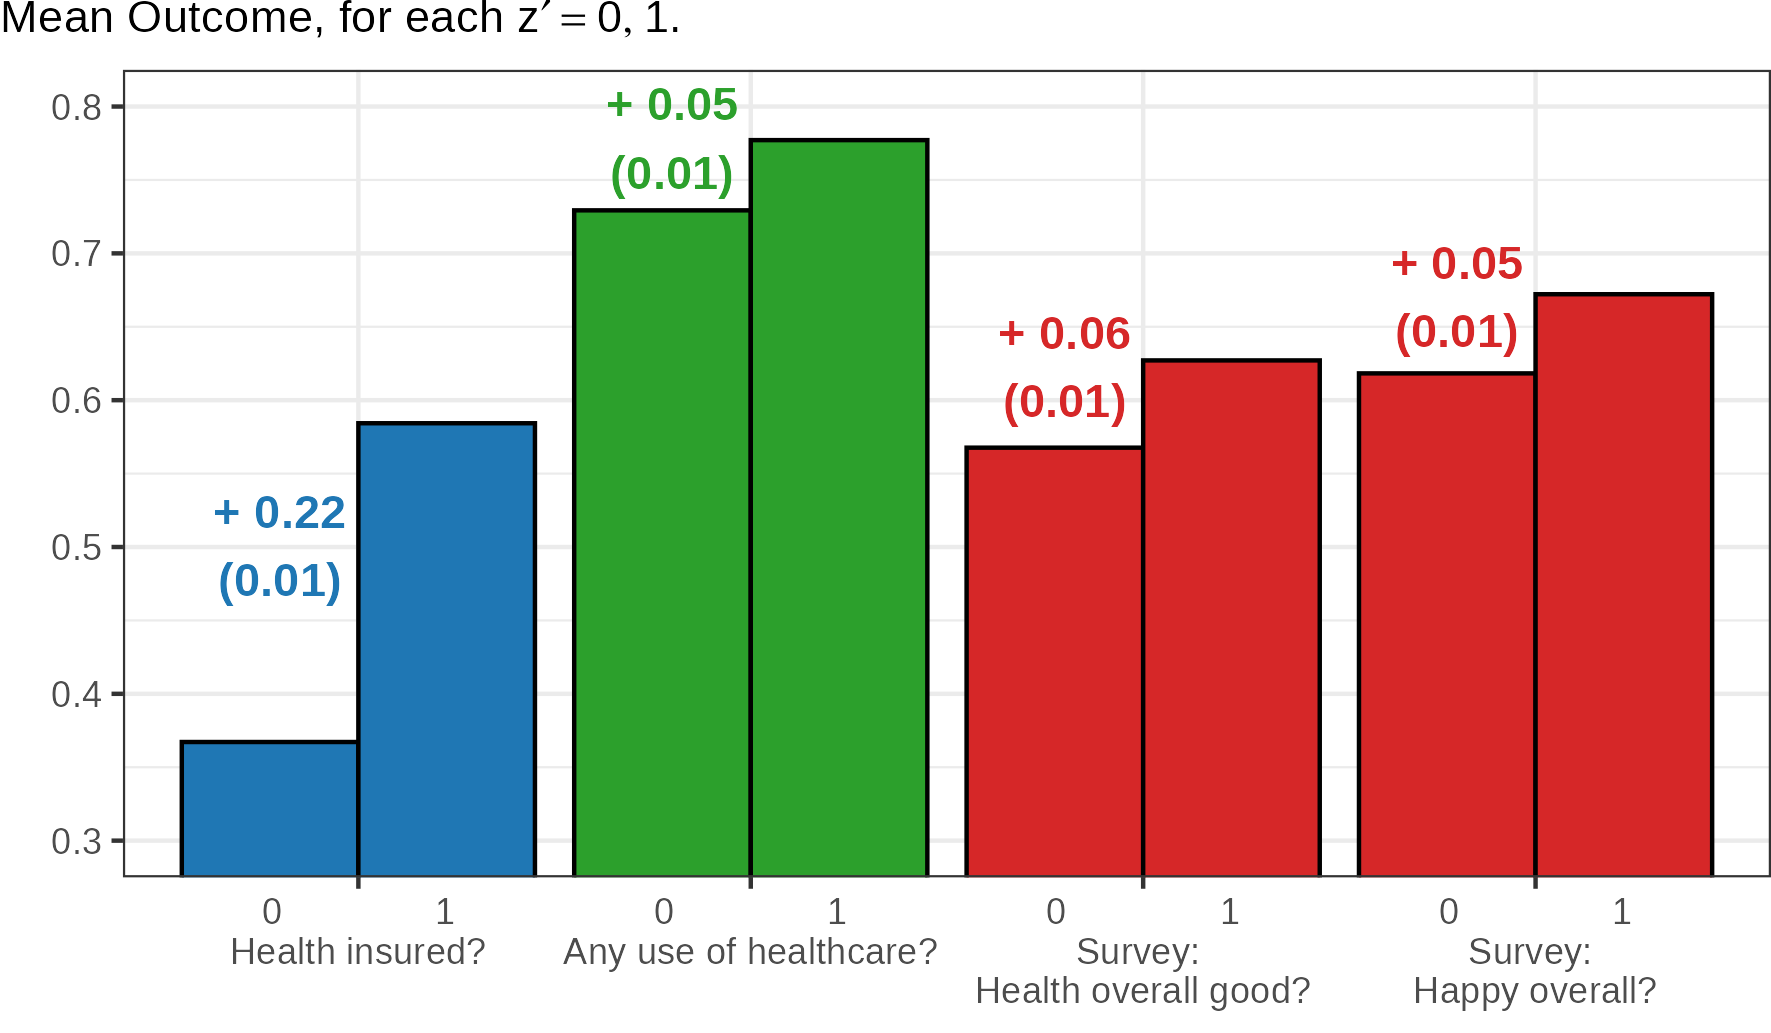
\includegraphics[width=0.85\textwidth]{
            presentation-files/figures/insurance-effects.png}
    \end{figure}
    \vspace{-0.5cm}

    \textbf{Applied practice:}

    $\Rightarrow$ Suggestive evidence for healthcare as mechanism for wait-list lottery….
\end{frame}
%-------------------------------------------------------------------------------
\begin{frame}[noframenumbering]
    \frametitle{Intro: Oregon Health Insurance Experiment}
    In 2008, Oregon gave access to socialised health insurance by wait-list lottery (Finkelstein et al, 2012).
    \begin{figure}
            \caption{Model for Suggestive Evidence of a Mechanism.}
            
\begin{tikzpicture}
            \node[state,thick,ForestGreen] (mediator) at (0,0) {$D_i$};
            \node[state,thick,blue] (treatment) [left=2cm of mediator] {$Z_i$};
            \node[state,thick,red] (outcome)   [right=2cm of mediator] {$Y_i$};
            % Label Z_i, D, Y_i
            \node[color=ForestGreen] [above=0.1cm of mediator] {Healthcare};
            \node[color=blue] [left=0.1cm of treatment] {Wait-list lottery};
            \node[color=red,align=left] [right=0.1cm of outcome] {Health \& \\ Happiness};
            % Draw the causal arrows
            \path[->, thick] (treatment) edge (mediator);
            %\path[->, dashed,color=gray] (mediator) edge (outcome);
            \path[->, thick] (treatment) edge[bend right=30] (outcome);
            % Label the problem.
            \node[color=RoyalPurple] [right=0.75cm of mediator] {?};
        \end{tikzpicture}
    \end{figure}
    \vfill
    \par\noindent\rule{\textwidth}{0.4pt}
    \textbf{Inconsistencies in this conclusion:}
    \begin{itemize}
        \item A triangular system missing the $D_i \to Y_i$ edge…
        \item Is $D_i \to Y_i$ small, large, or even existent?
        \item Where else do we accept assumed causal effects without evidence?
    \end{itemize}
\end{frame}
%-------------------------------------------------------------------------------
\begin{frame}
    \frametitle{Introduction}
    Causal Mediation (CM) is an alternative framework, which actually defines what is estimated, and assumptions under which they are identified.

    \par\noindent\rule{\textwidth}{0.4pt}
    This paper examines CM from an economic perspective:
    \begin{enumerate}
        \item Problems with conventional approach to CM in observational settings.
        \\ \textbf{[Negative result]}
        \item Recovering valid CM effects, via MTE $+$ control function modelling.
        \\ \textbf{[Positive result]}
    \end{enumerate}
    \par\noindent\rule{\textwidth}{0.4pt}
    Brings together ideas from two different literatures:
    \begin{itemize}
        \item \textbf{CM.}
        \\ {\small Imai Keele Yamamoto (2010), Fr\"olich Huber (2017), Deuchert Huber Schelker (2019), Huber (2020), Kwon Roth (2024).}
        \item \textbf{Labour theory, Selection-into-treatment, MTEs.}
        \\ {\small Roy (1951), Heckman (1979), Heckman Honor\'e (1990), Vycatil (2002), Heckman Vycatil (2005), Brinch Mogstad Wiswall (2017), Kline Walters (2019).}
    \end{itemize}
\end{frame}
%-------------------------------------------------------------------------------
\section{1. CM}
%-------------------------------------------------------------------------------
\begin{frame}
    \frametitle{1. CM --- Model}
    Consider binary \textcolor{blue}{treatment $Z_i = 0, 1$},
    binary \textcolor{ForestGreen}{mediator $D_i = 0, 1$},
    and continuous \textcolor{red}{outcome $Y_i$} for individuals $i = 1, \hdots, n$.
    \vskip-0.5cm
    \begin{figure}
        \centering
        \singlespacing
        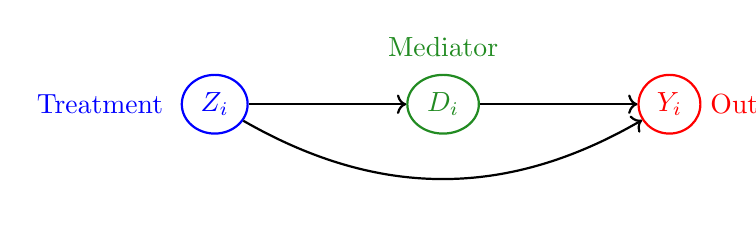
\begin{tikzpicture}
            \node[state, thick,ForestGreen] (mediator) at (0,0) {$D_i$};
            \node[state, thick,blue] (treatment) [left=2cm of mediator] {$Z_i$};
            \node[state, thick,red] (outcome) [right=2cm of mediator] {$Y_i$};
            % Label Z, D, Y
            \node[color=ForestGreen] [above=0.1cm of mediator] {Mediator};
            \node[color=blue] [left=0.1cm of treatment] {Treatment};
            \node[text width=0.1cm, color=red] [right=-0.01cm of outcome] {Outcome};
            % Draw the causal arrows
            \path[->, thick] (treatment) edge (mediator);
            \path[->, thick] (mediator) edge (outcome);
            \path[->, thick] (treatment) edge[bend right=30] (outcome);
            % Label direct and indirect effect
            %\node[color=orange] [above left=-0.35cm and 0.2cm of mediator] {First-stage};
            %\node[color=orange] [above right=-0.3cm and 0.4cm of mediator] {Indirect};
            %\node[color=orange] [below=0.5cm of mediator] {Direct Effect};
        \end{tikzpicture}
    \end{figure}
    Assume $Z_i$ is ignorable (conditional on $\vec X_i$).
    \par\noindent\rule{\textwidth}{0.4pt}
    \begin{align*}
        & \textcolor{ForestGreen}{\text{Mediator }D_i} \text{ is a function of } \textcolor{blue}{Z_i}.
        & \textcolor{red}{\text{Outcome }Y_i} \text{ is a function of both }
        \textcolor{blue}{Z_i}, \textcolor{ForestGreen}{D_i}. \\
        & D_i = \begin{cases}
            D_i(0), \text{ if } Z_i = 0 \\
            D_i(1), \text{ if } Z_i = 1.
        \end{cases}
        & Y_i = \begin{cases}
            Y_i(0, D_i(0)), \text{ if } Z_i = 0 \\
            Y_i(1, D_i(1)), \text{ if } Z_i = 1.
        \end{cases}
    \end{align*}
\end{frame}
%-------------------------------------------------------------------------------
\begin{frame}[noframenumbering]
    \frametitle{1. CM --- Model}
    Consider binary \textcolor{blue}{treatment $Z_i = 0, 1$},
    binary \textcolor{ForestGreen}{mediator $D_i = 0, 1$},
    and continuous \textcolor{red}{outcome $Y_i$} for individuals $i = 1, \hdots, n$.
    \vskip-0.5cm
    \begin{figure}
        \centering
        \singlespacing
        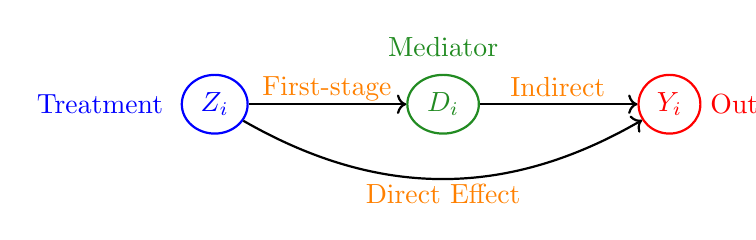
\begin{tikzpicture}
            \node[state, thick,ForestGreen] (mediator) at (0,0) {$D_i$};
            \node[state, thick,blue] (treatment) [left=2cm of mediator] {$Z_i$};
            \node[state, thick,red] (outcome) [right=2cm of mediator] {$Y_i$};
            % Label Z, D, Y
            \node[color=ForestGreen] [above=0.1cm of mediator] {Mediator};
            \node[color=blue] [left=0.1cm of treatment] {Treatment};
            \node[text width=0.1cm, color=red] [right=-0.01cm of outcome] {Outcome};
            % Draw the causal arrows
            \path[->, thick] (treatment) edge (mediator);
            \path[->, thick] (mediator) edge (outcome);
            \path[->, thick] (treatment) edge[bend right=30] (outcome);
            % Label direct and indirect effect
            \node[color=orange] [above left=-0.35cm and 0.2cm of mediator] {First-stage};
            \node[color=orange] [above right=-0.3cm and 0.4cm of mediator] {Indirect};
            \node[color=orange] [below=0.5cm of mediator] {Direct Effect};
        \end{tikzpicture}
    \end{figure}
    Assume $Z_i$ is ignorable (conditional on $\vec X_i$).
    \par\noindent\rule{\textwidth}{0.4pt}
    Only two causal effects are identified so far.
    \begin{align*}
    \text{ATE:} \;\; \E{Y_i(1, D_i(1)) - Y_i(0, D_i(0))}
        &= \Egiven{Y_i}{Z_i = 1} - \Egiven{Y_i}{Z_i = 0} \\
    \text{Average first-stage:} \;\; \E{D_i(1) - D_i(0)}
        &=\Egiven{D_i}{Z_i = 1} - \Egiven{D_i}{Z_i = 0}
    \end{align*}
\end{frame}
%-------------------------------------------------------------------------------
\begin{frame}[noframenumbering]
    \frametitle{1. CM --- Model}
    Consider binary \textcolor{blue}{treatment $Z_i = 0, 1$},
    binary \textcolor{ForestGreen}{mediator $D_i = 0, 1$},
    and continuous \textcolor{red}{outcome $Y_i$} for individuals $i = 1, \hdots, n$.
    \vskip-0.5cm
    \begin{figure}
        \centering
        \singlespacing
        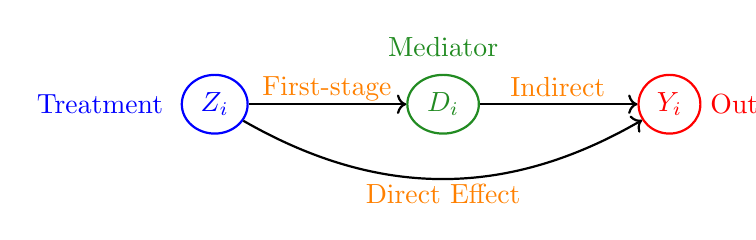
\begin{tikzpicture}
            \node[state, thick,ForestGreen] (mediator) at (0,0) {$D_i$};
            \node[state, thick,blue] (treatment) [left=2cm of mediator] {$Z_i$};
            \node[state, thick,red] (outcome) [right=2cm of mediator] {$Y_i$};
            % Label Z, D, Y
            \node[color=ForestGreen] [above=0.1cm of mediator] {Mediator};
            \node[color=blue] [left=0.1cm of treatment] {Treatment};
            \node[text width=0.1cm, color=red] [right=-0.01cm of outcome] {Outcome};
            % Draw the causal arrows
            \path[->, thick] (treatment) edge (mediator);
            \path[->, thick] (mediator) edge (outcome);
            \path[->, thick] (treatment) edge[bend right=30] (outcome);
            % Label direct and indirect effect
            \node[color=orange] [above left=-0.35cm and 0.2cm of mediator] {First-stage};
            \node[color=orange] [above right=-0.3cm and 0.4cm of mediator] {Indirect};
            \node[color=orange] [below=0.5cm of mediator] {Direct Effect};
        \end{tikzpicture}
    \end{figure}
    \vskip-0.5cm
    \par\noindent\rule{\textwidth}{0.4pt}
    \[ \text{Average Direct Effect (ADE)}: \;\;\;
        \E{Y_i\left(\eqhighlight{blue}{1}, D_i(Z_i) \right)
            - Y_i\left(\eqhighlight{blue}{0}, D_i(Z_i) \right)} \]
    \vskip-0.35cm
    \begin{itemize}
        \item ADE is causal effect $Z\to Y$, blocking the indirect $D_i$ path.
    \end{itemize}
    \vskip0.25cm
    \[ \text{Average Indirect Effect (AIE):} \;\;\;
    \E{Y_i\left(Z_i, \eqhighlight{ForestGreen}{D_i(1)} \right)
        - Y_i\left(Z_i, \eqhighlight{ForestGreen}{D_i(0)} \right)} \]
    \vskip-0.25cm
    \begin{itemize}
        \item AIE is causal effect of $D(Z) \to Y$, blocking the direct $Z_i$ path.
    \end{itemize}
\end{frame}
%-------------------------------------------------------------------------------
\begin{frame}
    \frametitle{1. CM --- Identification} 
    \textbf{Mediator Ignorability} (\textbf{MI}, Imai Keele Yamamoto 2010):
    \vskip0.125cm
    Assume \textcolor{ForestGreen}{mediator $D_i$} is \textit{also} ignorable, conditional on $\vec X_i$ and \textcolor{blue}{$Z_i$ realisation}
    \[ D_i \indep Y_i(z', d') \;\; | \;\; \vec X_i, Z_i = z',
        \text{ for } z', d' = 0, 1. \]
    \vskip-0.25cm
    \par\noindent\rule{\textwidth}{0.4pt}
    If \textbf{MI} holds then ADE and AIE are identified by two-stage regression:
    \makebox[\textwidth]{\parbox{1.25\textwidth}{
        \footnotesize
        \[ \E[D_i, \vec X_i]{
            \underbrace{\Egiven{Y_i}{Z_i = 1, D_i, \vec X_i} - \Egiven{Y_i}{Z_i = 0, D_i, \vec X_i}}_{\text{Second-stage regression, $Y_i$ on $Z_i$ holding $D_i, \vec X_i$ constant}}}
            = \text{ADE} \]
        \[ \E[Z_i, \vec X_i]{ \begin{aligned}&\underbrace{\Big(
            \Egiven{D_i}{Z_i = 1, \vec X_i} - \Egiven{D_i}{Z_i = 0, \vec X_i} \Big)}_{\text{First-stage regression, $D_i$ on $Z_i$}}\\
            &\times \underbrace{\Big(
            \Egiven{Y_i}{Z_i, D_i = 1, \vec X_i} - \Egiven{Y_i}{Z_i, D_i = 0, \vec X_i} \Big)}_{\text{Second-stage regression, $Y_i$ on $D_i$ holding $Z_i, \vec X_i$ constant}} \end{aligned}} = \text{AIE} \]
    }}
\end{frame}
%-------------------------------------------------------------------------------
\section{2. Selection Bias}
%-------------------------------------------------------------------------------
\begin{frame}
    \frametitle{2. Selection Bias}
    \textbf{Mediator ignorability} (\textbf{MI}, Imai Keele Yamamoto 2010):
    \vskip0.125cm
    Assume \textcolor{ForestGreen}{mediator $D_i$} is \textbf{\textit{also} ignorable}, conditional on $\vec X_i$, \textcolor{blue}{$Z_i$ realisation}
    \[ D_i \indep Y_i(z', d') \;\; | \;\; \vec X_i, Z_i = z',
        \text{ for } z', d' = 0, 1. \]
    \vskip-0.25cm
    \par\noindent\rule{\textwidth}{0.4pt}
    \colorbox{yellow}{Would this assumption hold true in settings economists study?}

    \vskip0.25cm    
    E.g., Oregon Health Insurance Experiment.
    \begin{figure}
        
\begin{tikzpicture}
            \node[state,thick,ForestGreen] (mediator) at (0,0) {$D_i$};
            \node[state,thick,blue] (treatment) [left=2cm of mediator] {$Z_i$};
            \node[state,thick,red] (outcome)   [right=2cm of mediator] {$Y_i$};
            % Label Z_i, D, Y_i
            \node[color=ForestGreen] [above=0.1cm of mediator] {Healthcare};
            \node[color=blue] [left=0.1cm of treatment] {Wait-list lottery};
            \node[color=red,align=left] [right=0.1cm of outcome] {Health \& \\ Happiness};
            % Draw the causal arrows
            \path[->, thick] (treatment) edge (mediator);
            \path[->, thick] (mediator) edge (outcome);
            \path[->, thick] (treatment) edge[bend right=30] (outcome);
        \end{tikzpicture}
    \end{figure}
    \begin{enumerate}
        \item Treatment is as-good-as random (2008 Oregon wait-list lottery).
        \item \colorbox{yellow}{Healthcare is quasi-random, conditional on lottery realisation $Z_i$} \\
        \colorbox{yellow}{and demographic controls $\vec X_i$ (no natural experiment...).}
    \end{enumerate}
\end{frame}
%-------------------------------------------------------------------------------
\begin{frame}
    \frametitle{2. Selection Bias}
    \colorbox{yellow}{Assume: Healthcare is quasi-random, conditional on lottery realisation $Z_i$} \\
        \colorbox{yellow}{and demographic controls $\vec X_i$ (no natural experiment...).}

    \par\noindent\rule{\textwidth}{0.4pt}
    Consider the case \textbf{individuals visit the doctor} to maximise health.
    \[ D_i \left( z' \right) = \indicator{
        \underbrace{C_i}_{\text{Costs}} \leq
        \underbrace{Y_i\left( z', 1 \right) - Y_i\left( z', 0 \right)}_{\text{Benefits}}}, \;\;\; \text{for } z'=0,1
    \]
    i.e., Roy (1951) selection-into-$D_i$.
    \par\noindent\rule{\textwidth}{0.4pt}
    \vfill
    \textbf{Theorem:}
    If selection is Roy-style, and benefits are not 100\% explained by $Z_i, \vec X_i$, then \textbf{MI} does not hold.

    \vskip0.125cm
    \textbf{Proof sketch:} suppose $D_i$ is ignorable $\implies$ selection-into-$D_i$ is explained 100\% by $\left\{ C_i, Z_i, \vec X_i \right\}$, while unobserved benefits explain 0\%.
\end{frame}
%-------------------------------------------------------------------------------
\begin{frame}[noframenumbering]
    \frametitle{2. Selection Bias}
    \colorbox{yellow}{Assume: Healthcare is quasi-random, conditional on lottery realisation $Z_i$} \\
        \colorbox{yellow}{and demographic controls $\vec X_i$ (no natural experiment...).}

    \vskip0.25cm
    Consider the case \textbf{individuals visit the doctor} to maximise health.
    \[ D_i \left( z' \right) = \indicator{
        \underbrace{C_i}_{\text{Costs}} \leq
        \underbrace{Y_i\left( z', 1 \right) - Y_i\left( z', 0 \right)}_{\text{Benefits}}}, \;\;\; \text{for } z'=0,1.
    \]
    i.e., Roy (1951) selection-into-$D_i$.
    \par\noindent\rule{\textwidth}{0.4pt}
    Roy selection-into-$D_i$ $\implies$ unobserved confounder $\vec U_i$ \\
    e.g., underlying health conditions.

    \vskip-1.75cm
    \makebox[\textwidth]{\parbox{1.25\textwidth}{
    \begin{figure}[h!]
        \centering
        \singlespacing
        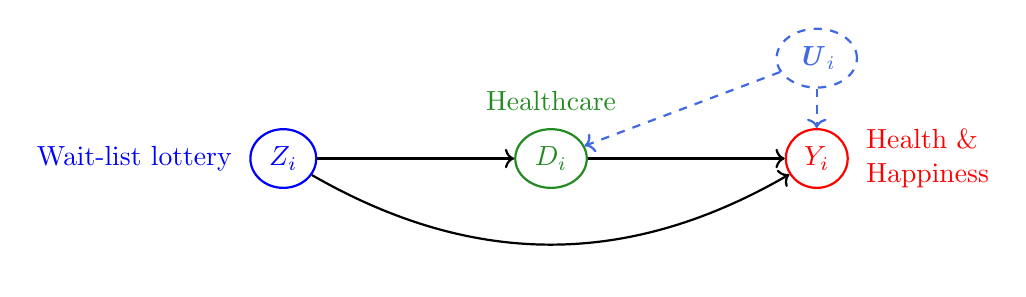
\begin{tikzpicture}
            \node[state, thick,ForestGreen] (mediator) at (0,0) {$D_i$};
            \node[state, thick,blue] (treatment) [left=2.5cm of mediator] {$Z_i$};
            \node[state, thick,red] (outcome) [right=2.5cm of mediator] {$Y_i$};
            % Label Z, D, Y
            \node[color=ForestGreen] [above=0.1cm of mediator] {Healthcare};
            \node[color=blue] [left=0.1cm of treatment] {Wait-list lottery};
            \node[color=red,align=left] [right=0.1cm of outcome] {Health \& \\ Happiness};
            % Draw the causal arrows
            \path[->, thick] (treatment) edge (mediator);
            \path[->, thick] (mediator) edge (outcome);
            \path[->, thick] (treatment) edge[bend right=30] (outcome);
            \node[state, thick,dashed,thick,RoyalBlue] (confounderU) [
                above=0.5cm of outcome] {$\vec U_i$};
            \path[->,thick,dashed,color=RoyalBlue] (confounderU) edge (mediator);
            \path[->,thick,dashed,color=RoyalBlue] (confounderU) edge (outcome);
            %\node[color=RoyalBlue] [right=0.1cm of confounderU] {Unobserved confounder};
        \end{tikzpicture}
    \end{figure}
    }}
\end{frame}
%-------------------------------------------------------------------------------
\begin{frame}
    \frametitle{2. Selection Bias}
    In observational setting, 
    must have an additional credible research design for \textbf{Mediator Ignorability (MI)} to believe this assumption.
    \vskip-0.5cm
    \begin{figure}[h!]
        \centering
        \singlespacing
        \begin{subfigure}[c]{0.475\textwidth}
            \centering
            \caption{Cells in a lab
                $\to$ \textbf{MI} believable.}
            
\includegraphics[width=\textwidth]{presentation-files/figures/science-lab.png}
        \end{subfigure}
        \begin{subfigure}[c]{0.475\textwidth}
            \centering
            \caption{People choosing healthcare
                $\to$ \textbf{MI} not.}
            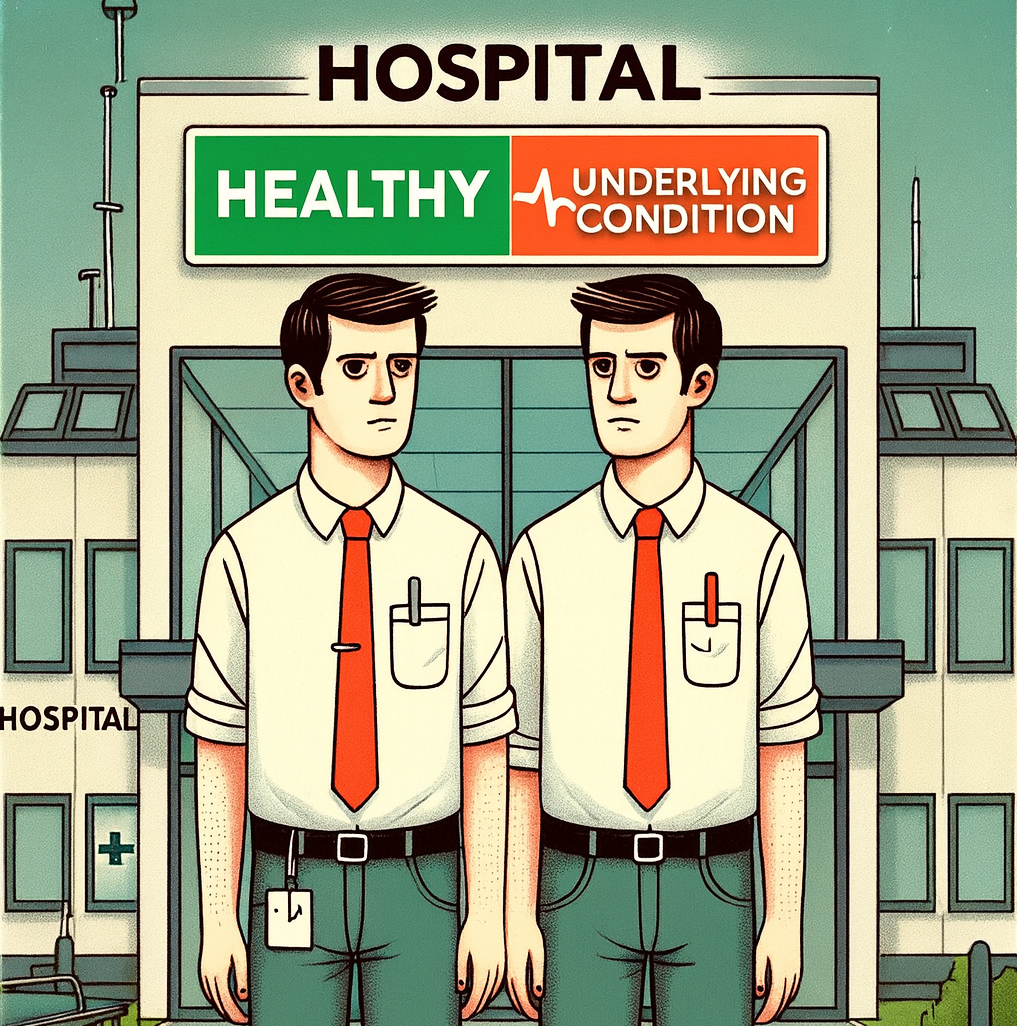
\includegraphics[width=0.965\textwidth]{presentation-files/figures/health-differences.png}
        \end{subfigure}
    \end{figure}
\end{frame}
%-------------------------------------------------------------------------------
\begin{frame}
    \frametitle{2. Selection Bias}
    \begin{itemize}
        \item What happens if you go ahead and estimate CM anyway?
        \item Would this be problematic?
        \item Estimating causal effects with an unobserved confounder is usually bad$\hdots$.
    \end{itemize}
    \par\noindent\rule{\textwidth}{0.4pt}
    \vskip0.25cm
    \textbf{Definition:} Selection bias (Heckman Ichimura Smith Todd, 1998).
    \vskip0.25cm
    Estimating $D_i \to Y_i$, if $D_i$ not ignorable:
    \begin{align*}
        &\Egiven{ Y_i}{D_i =1} - \Egiven{ Y_i}{D_i =0} \\
        &= \text{ATE} \\
        &\;\;\;\; + \underbrace{\Big(
            \Egiven{ Y_i(., 0)}{D_i =1} - \Egiven{ Y_i(.,0)}{D_i =0} \Big)}_{
                \text{\textcolor{red}{Selection Bias}}} \\
        &\;\;\;\;+ \underbrace{ \Prob{D_i=0} (\text{ATT}- \text{ATU}) }_{
            \text{\textcolor{orange}{Group difference bias}}}.
    \end{align*}
\end{frame}
%-------------------------------------------------------------------------------
\begin{frame}[noframenumbering]
    \frametitle{2. Selection Bias --- Direct Effect}
    \label{main:ade-selection-bias}
    CM Effects have this same flavour, causal effects $+$ contaminating bias.
    \[ \text{\textcolor{purple}{CM Estimand}}
        = \text{\textcolor{blue}{ADE}}
            + \Big(\text{\textcolor{red}{Selection Bias}}
            + \text{\textcolor{orange}{Group difference bias}}\Big)
        \hyperlink{cm-model}{\beamergotobutton{Model}} \]
    \vskip-0.25cm

    \par\noindent\rule{\textwidth}{0.4pt}
    {\footnotesize
    \begin{align*}
        & \underbrace{\mathbb E_{D_i=d'} \Big[
            \Egiven{Y_i}{Z_i = 1, D_i=d'} - \Egiven{Y_i}{Z_i = 0, D_i=d'} \Big]}_{
                \text{\textcolor{purple}{Estimand, Direct Effect}} } \\
        & = \underbrace{\E{Y_i(1, D_i(Z_i)) - Y_i(0, D_i(Z_i))}}_{
            \text{\textcolor{blue}{Average Direct Effect}}} \\
        & \;\;\;\; + 
        \underbrace{ \mathbb E_{D_i=d'} \Big[ 
            \Egiven{Y_i(0, D_i(Z_i))}{D_i(1) = d'} 
            - \Egiven{Y_i(0, D_i(Z_i))}{D_i(0) = d'} \Big] }_{
                \text{\textcolor{red}{Selection Bias}}} \\
        & \;\;\;\; + \underbrace{ \E[D_i =d']{
            \begin{aligned}
            &\Big(1 - \Prob{D_i(1) = d'} \Big) \\
            &\times \left( \begin{aligned}
                &\Egiven{Y_i(1, D_i(Z_i)) - Y_i(0, D_i(Z_i))}{D_i(1) = 1-d'} \\ 
                &  - \Egiven{Y_i(1, D_i(Z_i)) - Y_i(0, D_i(Z_i))}{D_i(0) = d'}
                \end{aligned} \right) \end{aligned}} }_{
                    \text{\textcolor{orange}{Group difference bias} 
                        \hyperlink{group-diff-ade}{\beamergotobutton{Group-diff}}}}
    \end{align*}}
\end{frame}
%-------------------------------------------------------------------------------
\begin{frame}[noframenumbering]
    \frametitle{2. Selection Bias --- Indirect Effect}
    \label{main:aie-selection-bias}
    CM Effects have this same flavour, causal effects $+$ contaminating bias.\footnote[frame]{
        Where $\bar\pi = \Prob{D_i(0) \neq D_i(1)}$, complier score.
    }
    \[ \text{\textcolor{purple}{CM Estimand}}
        = \text{\textcolor{ForestGreen}{AIE}}
            + \Big(\text{\textcolor{red}{Selection Bias}}
            + \text{\textcolor{orange}{Group difference bias}}\Big) \hyperlink{cm-model}{\beamergotobutton{Model}} \]
    \vspace{-0.5cm}

    \par\noindent\rule{\textwidth}{0.4pt}
    {\footnotesize
    \begin{align*}
        & \underbrace{\E[Z_i]{
            \Big( \Egiven{D_i}{Z_i = 1} - \Egiven{D_i}{Z_i = 0} \Big) \times
            \Big( \Egiven{Y_i}{Z_i, D_i = 1} - \Egiven{Y_i}{Z_i, D_i = 0} \Big) }}_{ \text{\textcolor{purple}{Estimand, Indirect Effect}} } \\
        & = \underbrace{\E{Y_i(Z_i, D_i(1)) - Y_i(Z_i, D_i(0))}}_{
            \text{\textcolor{ForestGreen}{Average Indirect Effect}} } \\
        & \;\;\;\; + \underbrace{\bar \pi  \Big(
            \Egiven{Y_i(Z_i, 0)}{D_i = 1} - \Egiven{Y_i(Z_i, 0)}{D_i = 0} \Big)}_{
                \text{\textcolor{red}{Selection Bias}}}\\
        & \;\;\;\; + \underbrace{ \bar\pi \left[ \begin{aligned}
            &\Big( 1 - \Prob{D_i=1} \Big)
            \left( \begin{aligned}
                &\Egiven{Y_i(Z_i, 1) - Y_i(Z_i, 0)}{D_i = 1} \\ 
                &  - \Egiven{Y_i(Z_i, 1) - Y_i(Z_i, 0)}{D_i = 0}
            \end{aligned} \right) \\
            &+ \left( \frac{1 - \Prob{D_i(1) = 1, D_i(0) = 0} }{
                \Prob{D_i(1) = 1, D_i(0) = 0}} \right)
            \left( \begin{aligned}
                &\Egiven{Y_i(Z_i, 1) - Y_i(Z_i, 0)}{D_i(Z_i) \neq Z_i} \\ 
                &  - \E{Y_i(Z_i, 1) - Y_i(Z_i, 0)}
            \end{aligned} \right)
        \end{aligned} \right]}_{\text{\textcolor{orange}{
            Groups difference Bias}
                \hyperlink{group-diff-aie}{\beamergotobutton{Group-diff}}}}
    \end{align*}}
\end{frame}
%-------------------------------------------------------------------------------
\begin{frame}
    \frametitle{2. Selection Bias}
    $\implies$ Unless mediator $D_i$ is also randomly assigned, then controlling for it does not lead to interpretable causal effects.
    \vskip0.25cm

    \par\noindent\rule{\textwidth}{0.4pt}
    \begin{enumerate}
        \item Counter to accepted intuitive reasoning in applied economics, which often controls for plausible mediators
        \item Invalidates conclusions in fields that uncritically apply CM methods with no case for mediator ignorability (common in some fields of epidemiology, psychology, medicine, and sociology)
        \item Warning sign for economists to avoid picking up this practice, and stop using it as a robustness check.
    \end{enumerate}
    \vfill
    \par\noindent\rule{\textwidth}{0.4pt}
    Applied economics would do better by thinking deeper on mediation.
\end{frame}
%-------------------------------------------------------------------------------
\section{3. CM with Selection}
%-------------------------------------------------------------------------------
\begin{frame}
    \frametitle{3. CM with Selection}
    Suppose $Z_i$ is ignorable, $D_i$ is not, so we have the following causal model.
    \vskip-0.75cm
    \begin{figure}
        \centering
        \singlespacing
        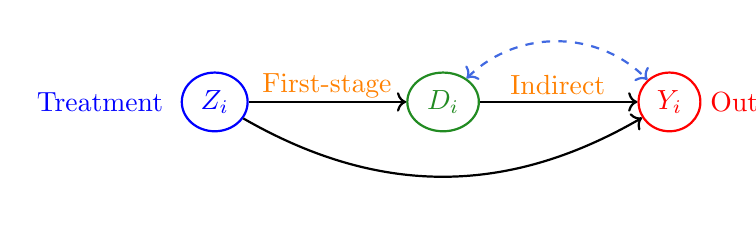
\begin{tikzpicture}
            \node[state, thick,ForestGreen] (mediator) at (0,0) {$D_i$};
            \node[state, thick,blue] (treatment) [left=2cm of mediator] {$Z_i$};
            \node[state, thick,red] (outcome) [right=2cm of mediator] {$Y_i$};
            % Label Z, D, Y
            %\node[color=ForestGreen] [above=0.1cm of mediator] {Mediator};
            \node[color=blue] [left=0.1cm of treatment] {Treatment};
            \node[text width=0.1cm, color=red] [right=-0.01cm of outcome] {Outcome};
            % Draw the causal arrows
            \path[->, thick] (treatment) edge (mediator);
            \path[->, thick] (mediator) edge (outcome);
            \path[->, thick] (treatment) edge[bend right=30] (outcome);
            % Label direct and indirect effect
            \node[color=orange] [above left=-0.35cm and 0.2cm of mediator] {First-stage};
            \node[color=orange] [above right=-0.3cm and 0.4cm of mediator] {Indirect};
            %\node[color=orange] [below=0.5cm of mediator] {Direct Effect};
            % Add in the unobserved confounding
            \path[<->,dashed,thick,color=RoyalBlue] (mediator) edge[bend right=-45] (outcome);
        \end{tikzpicture}
    \end{figure}
    \vskip-0.25cm
    \par\noindent\rule{\textwidth}{0.4pt}
    Write POs as sum of PO means and mean-zero errors, $U_{d', i}$.
    \[ Y_i(Z_i, 0)
        = \mu_0 \big( Z_i ;\vec X_i \big) + U_{0,i}, \;\;
    Y_i(Z_i, 1)
        = \mu_1 \big( Z_i ;\vec X_i \big) + U_{1,i}. \]
    \par\noindent\rule{\textwidth}{0.4pt}
    Then this system has the following random coefficient equations:
    \begin{align*}
        D_i &= \phi + \bar \pi Z_i + \varphi(\vec X_i) + U_i  \\
        Y_i &= \alpha + \beta D_i + \gamma Z_i + \delta Z_i D_i
        + \zeta(\vec X_i)
        + \underbrace{\eqhighlight{yellow}{
            \left(1 - D_i \right)U_{0,i} + D_i U_{1,i}}}_{
            \text{Correlated error term}}
    \end{align*}
    \vskip-0.5cm
    where $\beta, \gamma, \delta$ are functions of $\mu_{d'}(z'; \vec X_i)$.
\end{frame}
%-------------------------------------------------------------------------------
\begin{frame}[noframenumbering]
    \frametitle{3. CM with Selection}
    Suppose $Z_i$ is ignorable, $D_i$ is not, so we have the following causal model.
    \vskip-0.75cm
    \begin{figure}
        \centering
        \singlespacing
        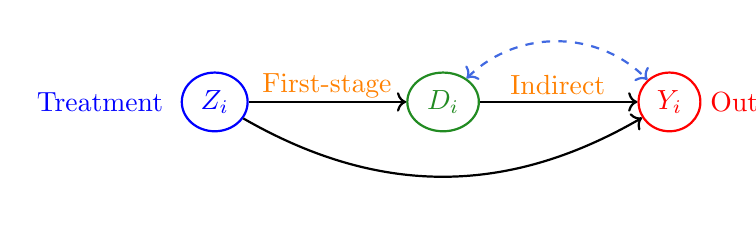
\begin{tikzpicture}
            \node[state, thick,ForestGreen] (mediator) at (0,0) {$D_i$};
            \node[state, thick,blue] (treatment) [left=2cm of mediator] {$Z_i$};
            \node[state, thick,red] (outcome) [right=2cm of mediator] {$Y_i$};
            % Label Z, D, Y
            %\node[color=ForestGreen] [above=0.1cm of mediator] {Mediator};
            \node[color=blue] [left=0.1cm of treatment] {Treatment};
            \node[text width=0.1cm, color=red] [right=-0.01cm of outcome] {Outcome};
            % Draw the causal arrows
            \path[->, thick] (treatment) edge (mediator);
            \path[->, thick] (mediator) edge (outcome);
            \path[->, thick] (treatment) edge[bend right=30] (outcome);
            % Label direct and indirect effect
            \node[color=orange] [above left=-0.35cm and 0.2cm of mediator] {First-stage};
            \node[color=orange] [above right=-0.3cm and 0.4cm of mediator] {Indirect};
            %\node[color=orange] [below=0.5cm of mediator] {Direct Effect};
            % Add in the unobserved confounding
            \path[<->,dashed,thick,color=RoyalBlue] (mediator) edge[bend right=-45] (outcome);
        \end{tikzpicture}
    \end{figure}
    \vskip-0.5cm
    
    \par\noindent\rule{\textwidth}{0.4pt}
    Then this system has the following random coefficient equations:
    \begin{align*}
        D_i &= \phi + \bar\pi Z_i + \varphi(\vec X_i) + U_i  \\
        Y_i &= \alpha + \beta D_i + \gamma Z_i + \delta Z_i D_i
        + \zeta(\vec X_i)
        + \underbrace{\eqhighlight{yellow}{
            \left(1 - D_i \right)U_{0,i} + D_i U_{1,i}}}_{
            \text{Correlated error term}}
    \end{align*}
    \vskip-0.5cm
    where $\beta, \gamma, \delta$ are functions of $\mu_{d'}(z'; \vec X_i)$.

    \par\noindent\rule{\textwidth}{0.4pt}
    \[ \text{ADE} = \E{\gamma + \delta D_i}, \;\;\;\;
    \text{AIE} = \E{ \bar \pi \big( \beta +  \delta Z_i + \tilde U_i \big)} \]
    with $\tilde U_i = \Egiven{ U_{1,i} - U_{0,i}}{
        \vec X_i, D_i(0) \neq D_i(1)}$ unobserved complier gains.
\end{frame}
%-------------------------------------------------------------------------------
\begin{frame}[noframenumbering]
    \frametitle{3. CM with Selection}
    Suppose $Z_i$ is ignorable, $D_i$ is not, so we have the following causal model.
    \vskip-0.75cm
    \begin{figure}
        \centering
        \singlespacing
        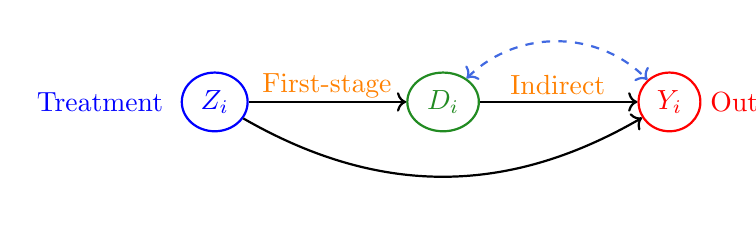
\begin{tikzpicture}
            \node[state, thick,ForestGreen] (mediator) at (0,0) {$D_i$};
            \node[state, thick,blue] (treatment) [left=2cm of mediator] {$Z_i$};
            \node[state, thick,red] (outcome) [right=2cm of mediator] {$Y_i$};
            % Label Z, D, Y
            %\node[color=ForestGreen] [above=0.1cm of mediator] {Mediator};
            \node[color=blue] [left=0.1cm of treatment] {Treatment};
            \node[text width=0.1cm, color=red] [right=-0.01cm of outcome] {Outcome};
            % Draw the causal arrows
            \path[->, thick] (treatment) edge (mediator);
            \path[->, thick] (mediator) edge (outcome);
            \path[->, thick] (treatment) edge[bend right=30] (outcome);
            % Label direct and indirect effect
            \node[color=orange] [above left=-0.35cm and 0.2cm of mediator] {First-stage};
            \node[color=orange] [above right=-0.3cm and 0.4cm of mediator] {Indirect};
            %\node[color=orange] [below=0.5cm of mediator] {Direct Effect};
            % Add in the unobserved confounding
            \path[<->,dashed,thick,color=RoyalBlue] (mediator) edge[bend right=-45] (outcome);
        \end{tikzpicture}
    \end{figure}
    \vskip-0.5cm
    
    \par\noindent\rule{\textwidth}{0.4pt}
    Main problem, second-stage is not identified:
    \begin{align*}
        \Egiven{Y_i}{Z_i, D_i, \vec X_i} \;\; =& \;\;
            \alpha
            + \beta D_i
            + \gamma Z_i
            + \delta Z_i D_i
            + \varphi(\vec X_i) \\
            & \;\; + \eqhighlight{yellow}{
                \left( 1 - D_i \right) \Egiven{ U_{0,i} }{D_i = 0, \vec X_i}} \\
            & \;\; + \underbrace{\eqhighlight{yellow}{
                D_i \Egiven{ U_{1,i} }{D_i = 1, \vec X_i}}}_{
                    \text{Unobserved $D_i$ confounding.}}
    \end{align*}
    \vfill

    \par\noindent\rule{\textwidth}{0.4pt}
    \textbf{Identification intuition:}
    Identify second-stage via MTE control function.
\end{frame}
%-------------------------------------------------------------------------------
\begin{frame}
    \frametitle{3. CM with Selection --- Identification}
    Assume:
    \begin{enumerate}
        \item Mediator monotonicity,
        $\Probgiven{ D_i(0) \leq D_i(1) }{\vec X_i} = 1$
        \[ \implies D_i(z') = \indicator{U_i \leq \pi(z'; \vec X_i)},
            \;\;\; \text{for } z'=0,1 \text{  (Vycatil 2002)}. \]
        \item Selection on mediator benefits,
        $\Cov{U_i, \, U_{0,i}}, \; \Cov{U_i, \, U_{1,i}} \neq 0$
        \[ \implies \text{First-stage take-up informs second-stage confounding.} \]
        \item There is an IV for the mediator, $\vec X_i^{\text{IV}}$ among control variables $\vec X_i$.
        \[ \implies \pi(Z_i ; \vec X_i) = \Probgiven{D_i = 1}{Z_i,\vec X_i} 
        \text{ is separately identified.} \]
    \end{enumerate}
    \par\noindent\rule{\textwidth}{0.4pt}
    \textbf{Proposition:}
    Under assumptions (1), (2), (3) the marginal effect of the mediator is identified,

    \vskip-0.5cm
    \begin{align*}
        & \Egiven{Y_i(z', 1) - Y_i(z', 0)}{Z_i = z', \vec X_i, U_i = p'} \\
        &= \beta + \delta z' + \Egiven{U_{1,i} - U_{0,i}}{\vec X_i, U_i = p'},
        \;\;\;\; \text{ for } p' \in (0,1).
    \end{align*}
\end{frame}
%-------------------------------------------------------------------------------
\begin{frame}
    \frametitle{3. CM with Selection --- Identification}
    The marginal effect has corresponding Control Functions (CFs), describing unobserved selection-into-$D_i$,
    \[ \rho_0 \lambda_0(p') = \Egiven{ U_{0,i} }{ p' \leq U_i }, \;\;\;\;
        \rho_1 \lambda_1(p') = \Egiven{ U_{1,i} }{ U_i \leq p' }. \]

    \vskip-0.25cm
    \par\noindent\rule{\textwidth}{0.4pt}
    These CFs restore second-stage identification, by extrapolating from $\vec X_i^{\text{IV}}$ compliers to $D_i(Z_i)$ mediator compliers,
    \begin{align*}
        \Egiven{Y_i}{Z_i, D_i, \vec X_i} \;\; =& \;\;
            \alpha
            + \beta D_i
            + \gamma Z_i
            + \delta Z_i D_i
            + \varphi(\vec X_i) \\
            & \;\; + \underbrace{\eqhighlight{yellow}{
                \rho_0 \left( 1 - D_i \right) \lambda_0 \big( \pi(Z_i ; \vec X_i) \big)
                + \rho_1 D_i \lambda_1 \big( \pi(Z_i ; \vec X_i) \big)}}_{
                    \text{CF adjustment.}}
    \end{align*}

    \par\noindent\rule{\textwidth}{0.4pt}
    This adjusted second-stage re-identifies the ADE and AIE,
    
    \makebox[\textwidth]{\parbox{1.25\textwidth}{
        \small
        \[ \text{ADE}
            = \E{\gamma + \delta D_i},
        \text{ AIE}
            = \mathbb E \Bigg[ \, \bar \pi \,
                \Big( \beta +  \delta Z_i +
                    \underbrace{ (\rho_1 - \rho_0) \,
                    \Gamma \big(\pi(0; \vec X_i), \, \pi(1; \vec X_i) \big)}_{
                        \text{Mediator compliers extrapolation.}} \Big) \Bigg] \]
    }}
\end{frame}
%-------------------------------------------------------------------------------
\begin{frame}
    \frametitle{3. CM with Selection --- Estimation}
    Will explain how estimation works, with simulation evidence.
    \vskip0cm
    \begin{enumerate}
        \item $\text{\textcolor{blue}{Random treatment $Z_i$}}
            \sim \text{Binom}\left(0.5 \right)$, for $n = 5,000$.
        \item $ \eqhighlight{yellow}{
            \left( U_{0,i}, U_{1,i} \right) \sim
        \text{BivariateNormal}\left( 0, 0, \sigma_0, \sigma_1, \rho \right)},
            \;\; \text{Costs }C_i \sim N(0, 0.5). $
    \end{enumerate}
    \par\noindent\rule{\textwidth}{0.4pt}
    Roy \textcolor{ForestGreen}{selection-into-$D_i$}, with constant partial effects $+$ interaction term.
    \begin{align*}
        D_i(z')    &= \indicator{C_i \leq Y_i(z', 1) - Y_i(z', 0)},&  \\
        Y_i(z',d') &= \left( z' + d' + z' d' \right) + U_{d'}
        & \text{ for } z',d' = 0,1.
    \end{align*}
    \par\noindent\rule{\textwidth}{0.4pt}
    Following the previous, these data have the following first and second-stage equations, where $\vec X_i^\text{IV}$ is an additive cost IV:
    \begin{align*}
        D_i &= \indicator{
            C_i - \Big( \eqhighlight{yellow}{U_{1,i} - U_{0,i}} \Big)
                \leq Z_i - \vec X_i^{\text{IV}} } \\
        Y_i &= Z_i + D_i + Z_i D_i
            + \eqhighlight{yellow}{
                \left( 1 - D_i \right) U_{0,i} + D_i U_{1,i}}.
    \end{align*}
    \small
    $\implies$ unobserved confounding by BivariateNormal $\Big(U_{0,i}, U_{1,i}\Big)$.
\end{frame}
%-------------------------------------------------------------------------------
\begin{frame}
    \frametitle{3. CM with Selection --- Estimation}
    Errors are normal, so system is Heckman (1979) selection model.

    \vskip0.25cm

    CFs are the inverse Mills ratio, with $\phi(.)$ normal pdf and $\Phi(.)$ normal cdf, 
    \[ \lambda_0(p') =
        \frac{\phi( - \Phi^{-1}(p') )}{\Phi( -\Phi^{-1}(p') )}, \;\;\;\;
    \lambda_1(p') =
        \frac{\phi( \Phi^{-1}(p') )}{\Phi( \Phi^{-1}(p') )},
        \;\;\;\; \text{ for } p' \in (0,1). \]

    \par\noindent\rule{\textwidth}{0.4pt}
    \textbf{Parametric Estimation Recipe:}
    \begin{enumerate}
        \item Estimate first-stage $\pi(Z_i; \vec X_i)$ with probit, including $\vec X_i^{\text{IV}}$.
        \item \hl{Include $\lambda_0, \lambda_1$ CFs in second-stage} OLS estimation.
        \item Compose CM estimates from two-stage plug-in estimates.
    \end{enumerate}
    \vfill

    \par\noindent\rule{\textwidth}{0.4pt}
    $\to$ Same as conventional CM estimates (two-stages), with CFs added.

    \makebox[\textwidth]{\parbox{1.25\textwidth}{
        \small
        \[ \hat{\text{ADE}}
            = \E{\hat\gamma + \hat\delta D_i}, \;\;
        \hat{\text{AIE}}
            = \mathbb E \Bigg[ \, \hat{\bar \pi} \,
                \Big( \hat\beta +  \hat\delta Z_i +
                    \underbrace{ (\hat\rho_1 - \hat\rho_0) \,
                    \Gamma \big(\hat\pi(0; \vec X_i), \, \hat\pi(1; \vec X_i) \big)}_{
                        \text{Mediator compliers extrapolation.}} \Big) \Bigg] \]
    }}
\end{frame}
%-------------------------------------------------------------------------------
\begin{frame}[noframenumbering]
    \frametitle{3. CM with Selection --- Estimation}
    \vskip-0.25cm
    \makebox[\textwidth]{\parbox{1.25\textwidth}{
        \begin{figure}
            \caption{Simulated Distribution of CM Effect Estimates from 10,000 DGPs.}
            \vskip-0.25cm
            \begin{subfigure}[c]{0.525\textwidth}
                \centering
                \caption{$\hat{\text{ADE}} - \text{ADE}$.}
                \vskip-0.25cm
                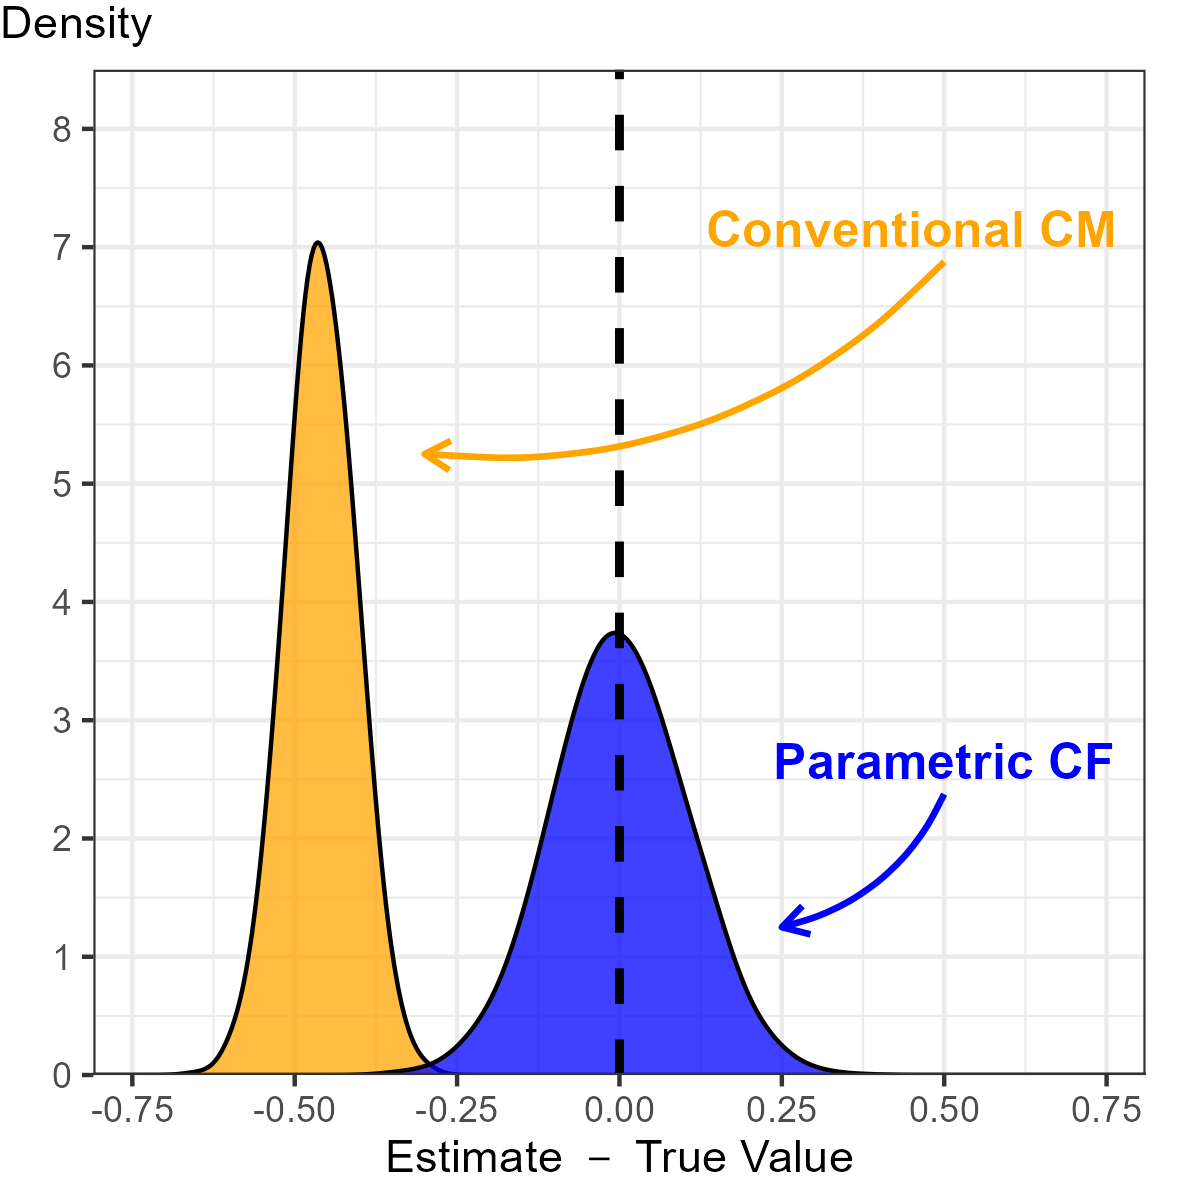
\includegraphics[width=\textwidth]{
                    ../text/sections/figures/normal-direct-dist.png}
            \end{subfigure}
            \begin{subfigure}[c]{0.525\textwidth}
                \centering
                \caption{$\hat{\text{AIE}} - \text{AIE}$.}
                \vskip-0.25cm
                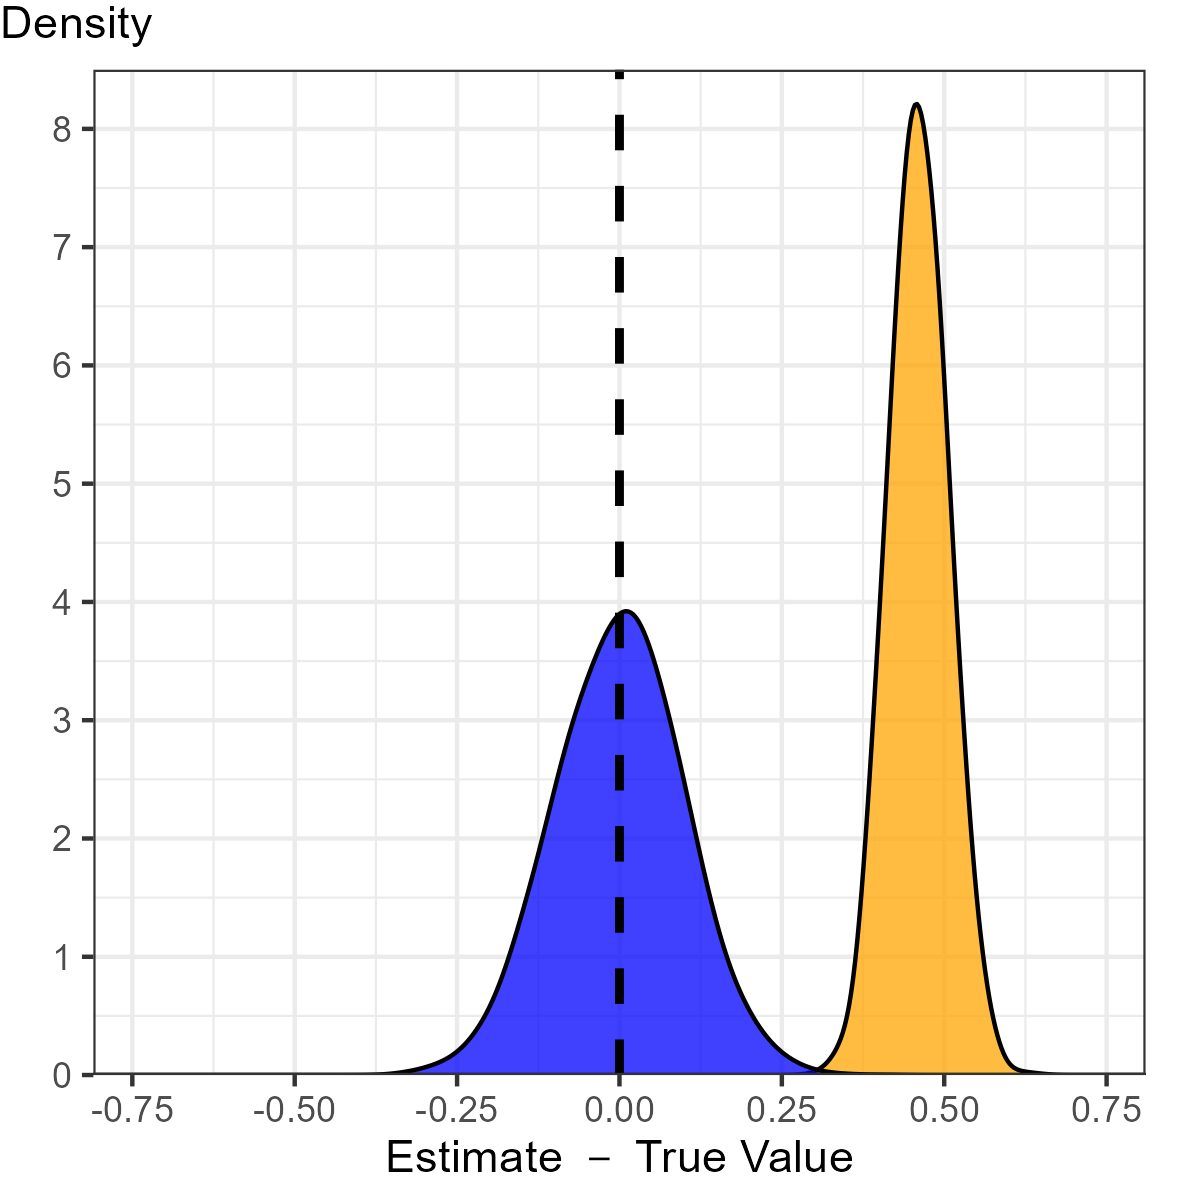
\includegraphics[width=\textwidth]{
                    ../text/sections/figures/normal-indirect-dist.png}
            \end{subfigure}
        \end{figure}
    }}
\end{frame}
%-------------------------------------------------------------------------------
\begin{frame}
    \frametitle{3. CM with Selection --- Estimation}
    If errors are not normal, then CFs do not have a known form, so semi-parametrically estimate them (e.g., splines).
    \begin{align*}
        \Egiven{Y_i}{Z_i, D_i = 0, \vec X_i} &=
            \alpha + \gamma Z_i + \varphi\big( \vec X_i \big)
            + \eqhighlight{yellow}{\rho_0 \lambda_0 \big( \pi(Z_i ; \vec X_i) \big)}, \\
        \Egiven{Y_i}{Z_i, D_i = 1, \vec X_i} &=
            (\alpha + \beta) + (\gamma + \delta) Z_i + \varphi\big( \vec X_i\big)
            + \eqhighlight{yellow}{\rho_1 \lambda_1 \big( \pi(Z_i ; \vec X_i) \big)}.
    \end{align*}

    \par\noindent\rule{\textwidth}{0.4pt}
    \textbf{Semi-parametric Estimation Recipe:}
    \begin{enumerate}
        \item Estimate first-stage $\pi(Z_i; \vec X_i)$, including $\vec X_i^{\text{IV}}$.
        \item \hl{Estimate second-stage separately for $D_i = 0$ and $D_i = 1$, with regressors $\lambda_0(p'), \lambda_1(p')$,} semi-parametric in $\hat\pi(Z_i; \vec X_i)$.
        \item Compose CM estimates from two-stage plug-in estimates. 
    \end{enumerate}
    \vfill

    \par\noindent\rule{\textwidth}{0.4pt}
    $\to$ Same as conventional CM estimates, with semi-parametric CFs.
    \hyperlink{cf-semiparametric}{\beamergotobutton{CFs.}}
    
    \vskip0.125cm
    \makebox[\textwidth]{\parbox{1.25\textwidth}{
        \small
        \[ \hat{\text{ADE}}
            = \E{\hat\gamma + \hat\delta D_i}, \;\;
        \hat{\text{AIE}}
            = \mathbb E \Bigg[ \, \hat{\bar \pi} \,
                \Big( \hat\beta +  \hat\delta Z_i +
                    (\hat\rho_1 - \hat\rho_0) \,
                    \Gamma \big(\hat\pi(0; \vec X_i), \, \hat\pi(1; \vec X_i) \big)\Big) \Bigg] \]
    }}
\end{frame}
%-------------------------------------------------------------------------------
\begin{frame}[noframenumbering]
    \frametitle{3. CM with Selection --- Estimation}
    \vskip-0.25cm
    \makebox[\textwidth]{\parbox{1.25\textwidth}{
        \begin{figure}
            \caption{Simulated Distribution of CM Effect Estimates with Uniform Errors.}
            \vskip-0.25cm
            \begin{subfigure}[c]{0.525\textwidth}
                \centering
                \caption{$\hat{\text{ADE}} - \text{ADE}$.}
                \vskip-0.25cm
                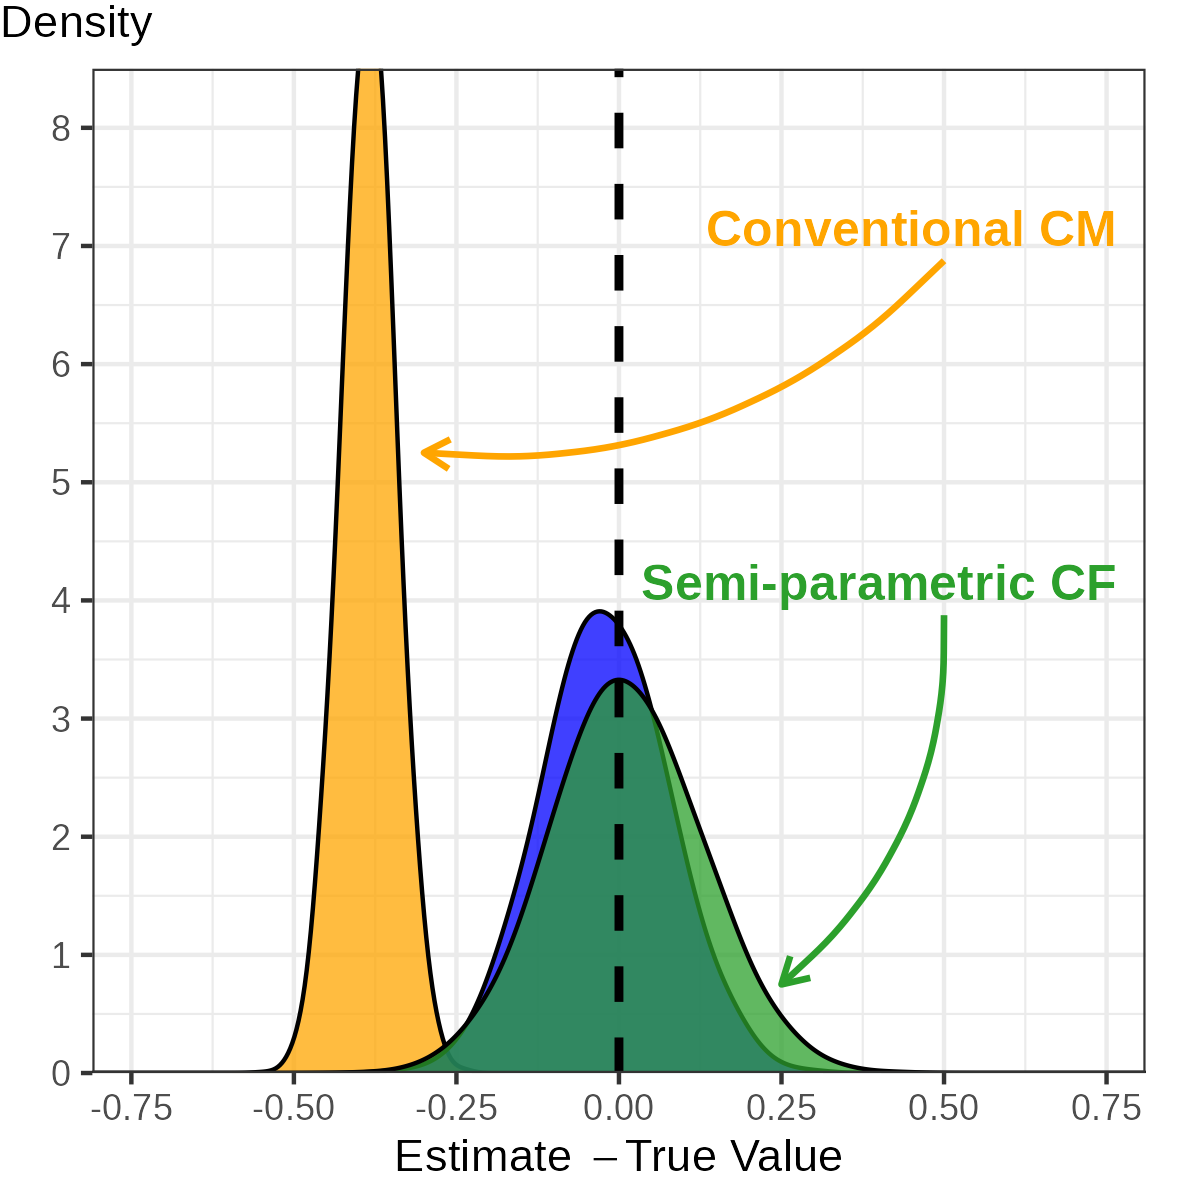
\includegraphics[width=\textwidth]{
                    ../text/sections/figures//uniform-direct-dist.png}
            \end{subfigure}
            \begin{subfigure}[c]{0.525\textwidth}
                \centering
                \caption{$\hat{\text{AIE}} - \text{AIE}$.}
                \vskip-0.25cm
                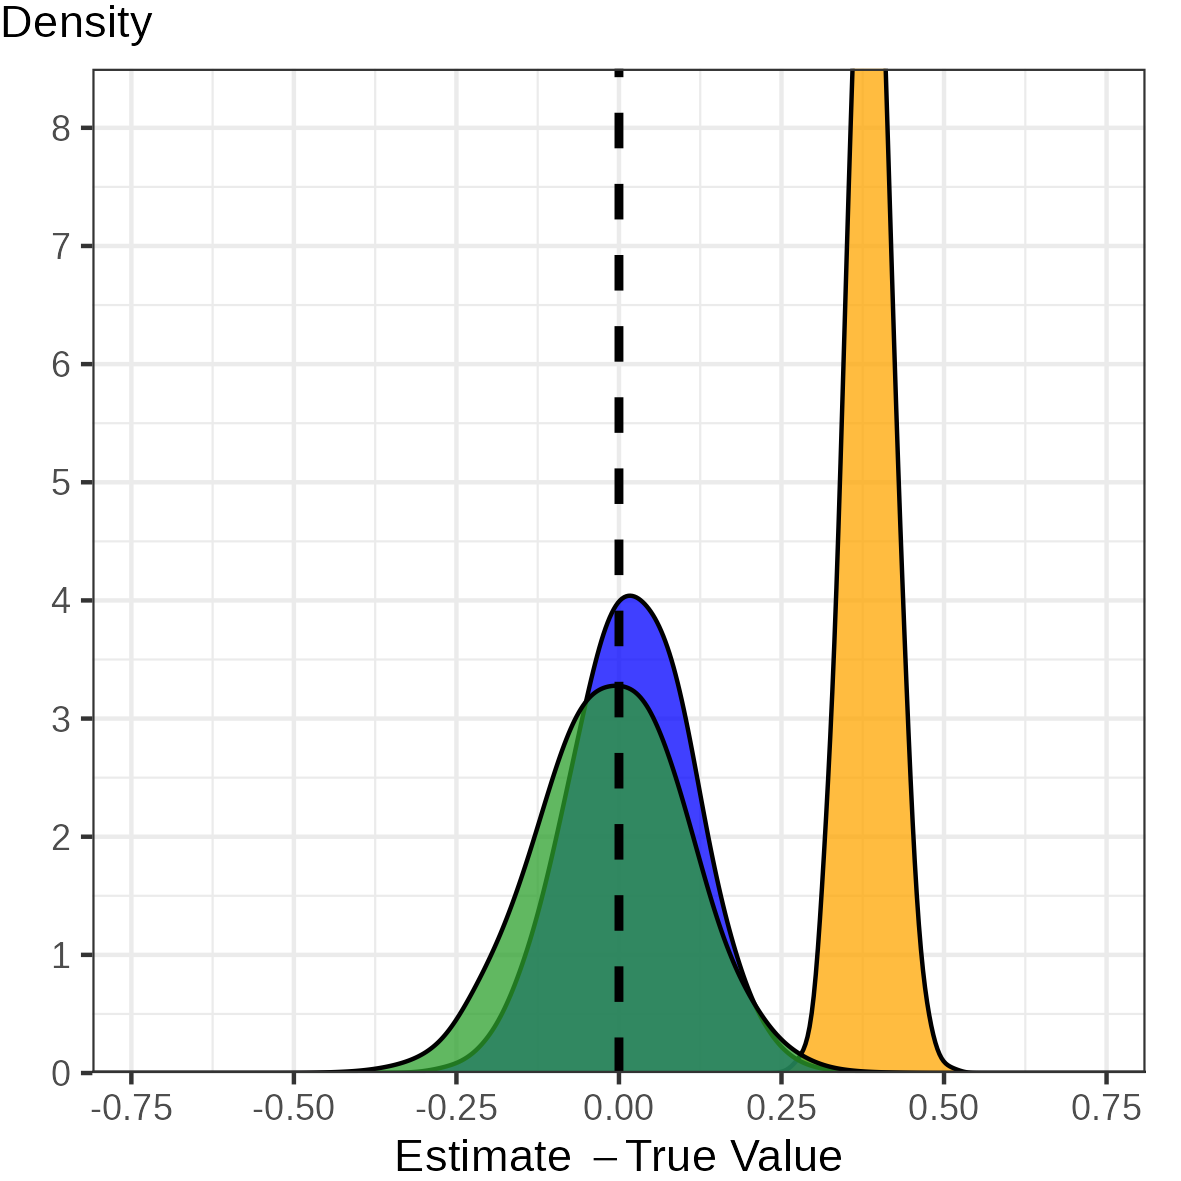
\includegraphics[width=\textwidth]{
                    ../text/sections/figures//uniform-indirect-dist.png}
            \end{subfigure}
        \end{figure}
    }}
\end{frame}
%-------------------------------------------------------------------------------
\begin{frame}[noframenumbering]
    \frametitle{3. CM with Selection --- Estimation}
    \vskip-0.25cm
    \makebox[\textwidth]{\parbox{1.25\textwidth}{
        \begin{figure}
            \caption{CF Adjusted Estimates Work with Different Error Term Parameters.}
            \vskip-0.25cm
            \begin{subfigure}[c]{0.525\textwidth}
                \centering
                \caption{ADE.}
                \vskip-0.25cm
                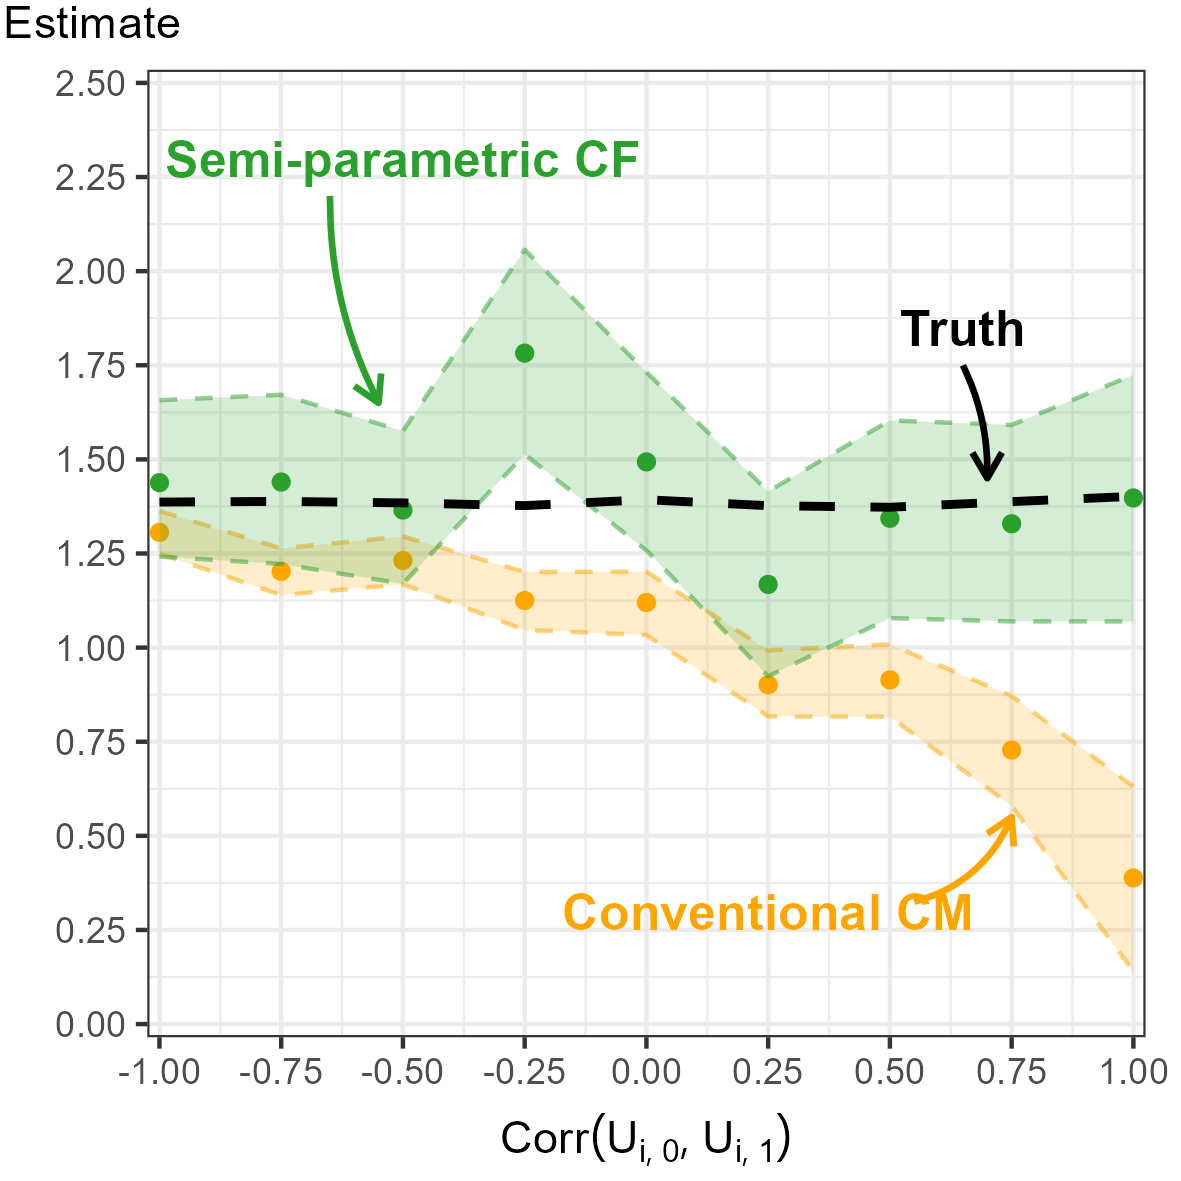
\includegraphics[width=\textwidth]{
                    ../text/sections/figures//rho-directeffect-bias.png}
            \end{subfigure}
            \begin{subfigure}[c]{0.525\textwidth}
                \centering
                \caption{AIE.}
                \vskip-0.25cm
                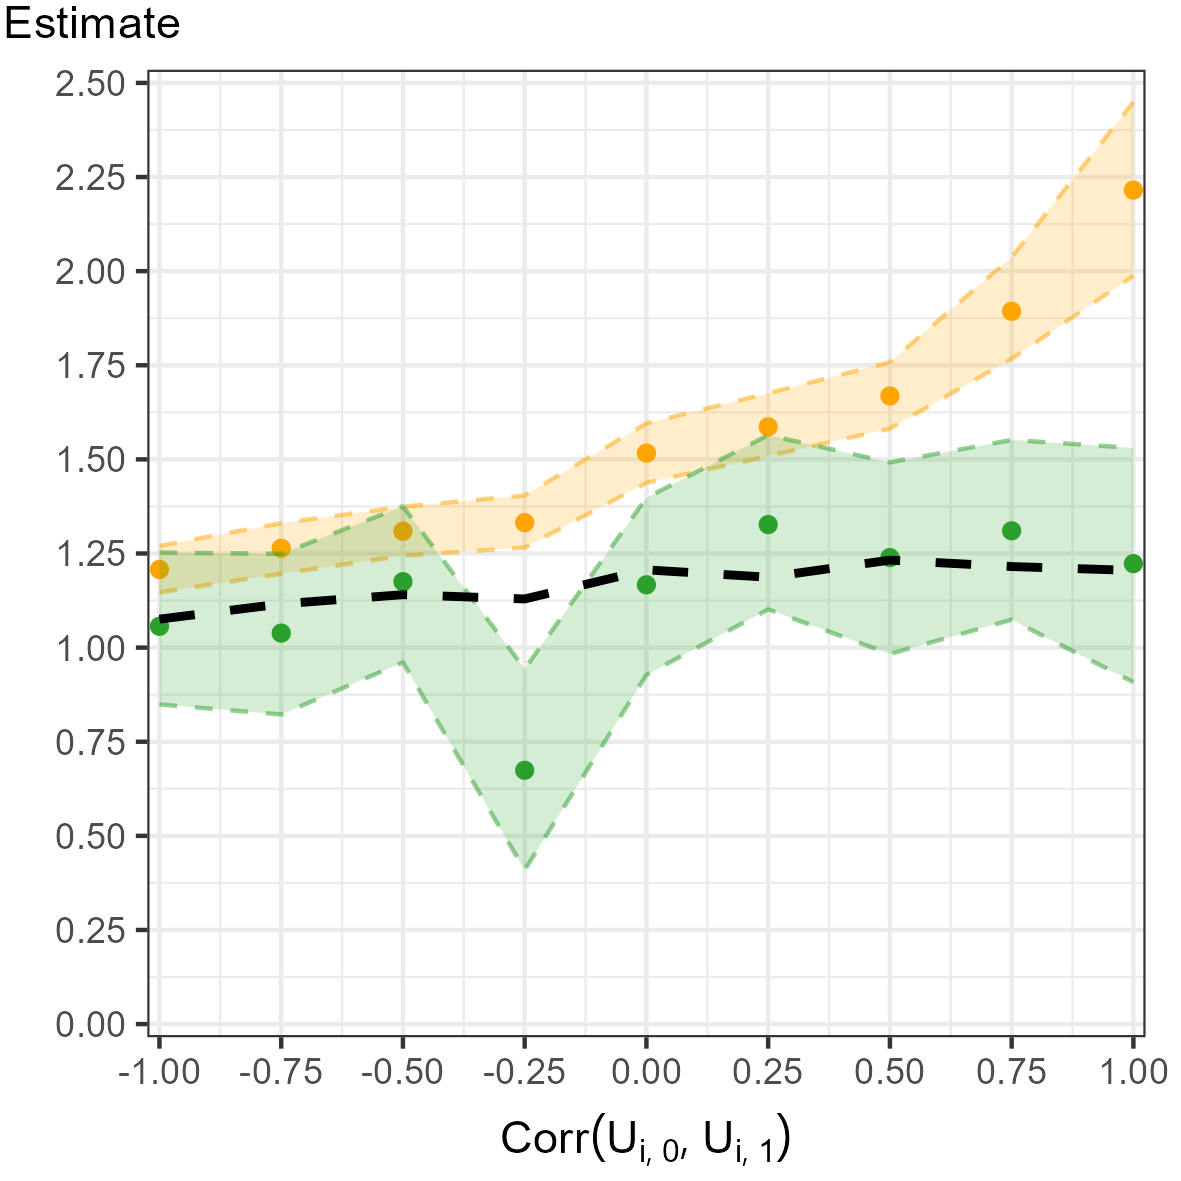
\includegraphics[width=\textwidth]{
                    ../text/sections/figures//rho-indirecteffect-bias.png}
            \end{subfigure}
        \end{figure}
    }}
\end{frame}
%-------------------------------------------------------------------------------
\section{Conclusion}
%-------------------------------------------------------------------------------
\begin{frame}
    \frametitle{Conclusion}
    \textbf{Overarching goals:}
    \begin{enumerate}
        \item Alternative to practice of suggestive evidence for mechanisms.
        \item Selection bias in conventional CM analyses with no case for mediator ignorability \\
        $\to$ Noted problems in the most popular methods for CM, pertinent for economic applications.
        \item Connect CM with labour theory $+$ selection-into-treatment $+$ MTEs \\
        $\to$ Valid CM identification in these settings.
    \end{enumerate}
    \par\noindent\rule{\textwidth}{0.4pt}
    \small
    \textbf{Caveats and points to remember:}
    \begin{itemize}
        \item Structural assumptions and IV for identification $+$ estimation (not ideal).
        \item Application to Oregon Health Insurance Experiment in the paper, showing health $+$ well-being effects mediated by healthcare (wide confidence intervals).
        \item \hl{\textbf{Credible} CM analyses are hard in practice.}
    \end{itemize}
\end{frame}
%-------------------------------------------------------------------------------
\section{Appendix}
%-------------------------------------------------------------------------------
\begin{frame}[noframenumbering]
    \frametitle{Appendix: CM Guiding Model}
    \label{cm-model}
    Consider binary \textcolor{blue}{treatment $Z_i = 0, 1$},
    binary \textcolor{ForestGreen}{mediator $D_i = 0, 1$},
    and continuous \textcolor{red}{outcome $Y_i$} for individuals $i = 1, \hdots, n$.
    \vskip-1.00cm
    \begin{figure}[h!]
        \centering
        \singlespacing
        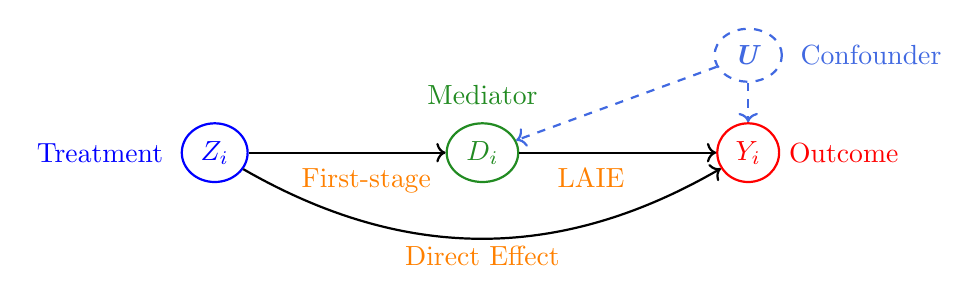
\begin{tikzpicture}
            \node[state, thick,ForestGreen] (mediator) at (0,0) {$D_i$};
            \node[state, thick,blue] (treatment) [left=2.5cm of mediator] {$Z_i$};
            \node[state, thick,red] (outcome) [right=2.5cm of mediator] {$Y_i$};
            % Label Z, D, Y
            \node[color=ForestGreen] [above=0.1cm of mediator] {Mediator};
            \node[color=blue] [left=0.1cm of treatment] {Treatment};
            \node[text width=0.1cm, color=red] [right=-0.01cm of outcome] {Outcome};
            % Draw the causal arrows
            \path[->, thick] (treatment) edge (mediator);
            \path[->, thick] (mediator) edge (outcome);
            \path[->, thick] (treatment) edge[bend right=30] (outcome);
            % Label direct and indirect effect
            \node[color=orange] [below left=-0.2cm and 0.2cm of mediator] {First-stage};
            \node[color=orange] [below right=-0.2cm and 0.5cm of mediator] {LAIE};
            \node[color=orange] [below=0.675cm of mediator] {Direct Effect};
            % Add in the confounders
            %\node[state, thick,RoyalPurple] (confounderX) [above=1.5cm of mediator] {$\vec{X}$};
            %\path[->,RoyalPurple] (confounderX) edge (mediator);
            %\node[color=RoyalPurple] [left=0.1cm of confounderX] {Observed controls};
            \node[state, thick,dashed,thick,RoyalBlue] (confounderU) [
                above=0.5cm of outcome] {$\vec U$};
            \node[color=RoyalBlue] [right=0.1cm of confounderU] {Confounder};
            \path[->,thick,dashed,color=RoyalBlue] (confounderU) edge (mediator);
            \path[->,thick,dashed,color=RoyalBlue] (confounderU) edge (outcome);
            %\node[color=RoyalBlue] [right=0.1cm of confounderU] {Unobserved confounder};
        \end{tikzpicture}
    \end{figure}
    \vskip-0.5cm
    \par\noindent\rule{\textwidth}{0.4pt}
    \[ \text{Average Direct Effect (ADE)}: \;\;\;
        \E{Y_i\left(\eqhighlight{blue}{1}, D_i(Z_i) \right)
            - Y_i\left(\eqhighlight{blue}{0}, D_i(Z_i) \right)} \]
    \vskip-0.35cm
    \begin{itemize}
        \item ADE is causal effect $Z\to Y$, blocking the indirect $D_i$ path.
    \end{itemize}
    \vskip0.25cm
    \[ \text{Average Indirect Effect (AIE):} \;\;\;
    \E{Y_i\left(Z_i, \eqhighlight{ForestGreen}{D_i(1)} \right)
        - Y_i\left(Z_i, \eqhighlight{ForestGreen}{D_i(0)} \right)} \]
    \vskip-0.25cm
    \begin{itemize}
        \item AIE is causal effect of $D(Z) \to Y$, blocking the direct $Z_i$ path.
    \end{itemize}
\end{frame}
%-------------------------------------------------------------------------------
\begin{frame}[noframenumbering]
    \frametitle{Group Difference --- ADE}
    \label{group-diff-ade}
    CM effects contaminated by (less interpretable) bias terms.
    \[ \text{\textcolor{purple}{CM Estimand}}
        = \text{\textcolor{blue}{ADEM}}
            + \text{\textcolor{red}{Selection Bias}} \]
    \vspace{-0.25cm}
    {\footnotesize
    \begin{align*}
        & \underbrace{\mathbb E_{D_i} \Big[
            \Egiven{Y_i}{Z_i = 1, D_i} - \Egiven{Y_i}{Z_i = 0, D_i} \Big]}_{
                \text{\textcolor{purple}{Estimand, Direct Effect}} } \\
        & = \underbrace{\E[D_i= d']{
            \Egiven{Y_i(1, D_i(Z_i)) - Y_i(0, D_i(Z_i))}{D_i(1) = d'}} }_{
            \text{\textcolor{blue}{Average Direct Effect on Mediator (ADEM) take-up --- i.e., $D_i(1)$ weighted}}} \\
        & \;\;\;\; + \underbrace{ \mathbb E_{D_i} \Big[ 
            \Egiven{Y_i(0, D_i(Z_i))}{D_i(1) = d'} 
            - \Egiven{Y_i(0, D_i(Z_i))}{D_i(0) = d'} \Big] }_{
                \text{\textcolor{red}{Selection Bias}}}
    \end{align*}}
    The weighted ADE you get here is a positive weighted sum of local ADEs, but with policy irrelevant weights $D_i(1) = d'$.

    \vskip0.5cm
    $\implies$ consider this group bias, noting difference from true ADE.
    \hyperlink{main:ade-selection-bias}{\beamergotobutton{Back}}
\end{frame}
%-------------------------------------------------------------------------------
\begin{frame}[noframenumbering]
    \frametitle{Group Difference --- AIE}
    \label{group-diff-aie}
    CM effects contaminated by (less interpretable) bias terms.
    \[ \text{\textcolor{purple}{CM Estimand}}
        = \text{\textcolor{ForestGreen}{AIEM}}
            + \Big(\text{\textcolor{red}{Selection Bias}}
            + \text{\textcolor{orange}{Group difference bias}}\Big) \]
    \vspace{-0.25cm}
    {\footnotesize
    \begin{align*}
        & \underbrace{\E[Z_i]{
            \Big( \Egiven{D_i}{Z_i = 1} - \Egiven{D_i}{Z_i = 0} \Big) \times
            \Big( \Egiven{Y_i}{Z_i, D_i = 1} - \Egiven{Y_i}{Z_i, D_i = 0} \Big) }}_{ \text{\textcolor{purple}{Estimand, Indirect Effect}} } \\
        & = \underbrace{
                \Egiven{Y_i(Z_i, D_i(1)) - Y_i(Z_i, D_i(0))}{D_i = 1}
            }_{\text{\textcolor{ForestGreen}{Average Indirect Effect on Mediated (AIEM) --- i.e., $D_i=1$ weighted}} } \\
        & \;\;\;\; + \underbrace{\bar \pi  \Big(
            \Egiven{Y_i(Z_i, 0)}{D_i = 1} - \Egiven{Y_i(Z_i, 0)}{D_i = 0} \Big)}_{
                \text{\textcolor{red}{Selection Bias}}} \\
        & \;\;\;\; + \underbrace{\bar \pi \left[
            \left( \frac{1 - \Prob{D_i(1) = 1, D_i(0) = 0} }{
                \Prob{D_i(1) = 1, D_i(0) = 0}} \right)
            \left( \begin{aligned}
                &\Egiven{Y_i(Z_i, 1) - Y_i(Z_i, 0)}{D_i(1) = 0 \text{ or } D_i(0)=1} \\ 
                &  - \E{Y_i(Z_i, 1) - Y_i(Z_i, 0)}
            \end{aligned} \right)
        \right]}_{\text{\textcolor{orange}{Groups difference Bias}}}
    \end{align*}}
    The weighted AIE you get here is not a positive weighted sum of local AIEs, 
    because the AIE is only about $D(Z)$ compliers.
    \hyperlink{cm-model}{\beamergotobutton{Model}}.

    $\implies$ consider this group bias, noting difference from true AIE.
    \hyperlink{main:aie-selection-bias}{\beamergotobutton{Back}}
\end{frame}
%-------------------------------------------------------------------------------
\begin{frame}[noframenumbering]
    \frametitle{Semi-parametric Control Functions}
    \label{cf-semiparametric}
    Semi-parametric specifications for the CFs $\lambda_0, \lambda_1$ bring some complications to estimating the AIE.
    \begin{align*}
        \Egiven{Y_i}{Z_i, D_i = 0, \vec X_i} &=
            \alpha + \gamma Z_i + \varphi\big( \vec X_i \big)
            + \eqhighlight{yellow}{\rho_0 \lambda_0 \big( \pi(Z_i ; \vec X_i) \big)}, \\
        \Egiven{Y_i}{Z_i, D_i = 1, \vec X_i} &=
            (\alpha + \beta) + (\gamma + \delta) Z_i + \varphi\big( \vec X_i\big)
            + \eqhighlight{yellow}{\rho_1 \lambda_1 \big( \pi(Z_i ; \vec X_i) \big)}.
    \end{align*}
    Intercepts, $\alpha, (\alpha + \beta)$, and relevance parameters $\rho_0, \rho_1$ are not separately identified from the CFs $\lambda_0(.), \lambda_1(.)$ so CF extrapolation term\\ $(\rho_1 - \rho_0) \Gamma \big(\pi(0; \vec X_i), \, \pi(1; \vec X_i) \big)$ is not directly identified or estimable.

    \par\noindent\rule{\textwidth}{0.4pt}    
    These problems can be avoided by estimating the AIE using its relation to the ATE, $\hat{\text{AIE}}^{\text{CF}} =$
    \[ \hat{\text{ATE}}
        - (1 - \bar Z) \, \underbrace{\left( 
            \frac 1N \sum_{i = 1}^N \hat\gamma + \hat \delta \, \hat\pi(1; \vec X_i) \right)}_{\hat{\text{ADE}}\text{ given }Z_i = 1}
        - \bar Z \, \underbrace{\left(
            \frac 1N \sum_{i = 1}^N \hat\gamma + \hat \delta \, \hat\pi(0; \vec X_i)  \right)}_{\hat{\text{ADE}}\text{ given }Z_i = 0}. \]
\end{frame}
%-------------------------------------------------------------------------------
\end{document}
